\documentclass[10pt,psamsfonts]{amsart}

%-------Packages---------
\usepackage{amssymb,amsfonts}
%\usepackage[all,arc]{xy}
\usepackage{enumerate}
%\usepackage{mathrsfs}
\usepackage{subcaption}
\usepackage{graphicx}
\usepackage{caption}
\usepackage[margin=0.2in]{geometry}
\usepackage{wrapfig}

%--------Theorem Environments--------
%theoremstyle{plain} --- default
\newtheorem{thm}{Theorem}[section]
\newtheorem{cor}[thm]{Corollary}
\newtheorem{prop}[thm]{Proposition}
\newtheorem{lem}[thm]{Lemma}
\newtheorem{conj}[thm]{Conjecture}
\newtheorem{quest}[thm]{Question}

\theoremstyle{definition}
\newtheorem{defn}[thm]{Definition}
\newtheorem{defns}[thm]{Definitions}
\newtheorem{con}[thm]{Construction}
\newtheorem{exmp}[thm]{Example}
\newtheorem{exmps}[thm]{Examples}
\newtheorem{notn}[thm]{Notation}
\newtheorem{notns}[thm]{Notations}
\newtheorem{addm}[thm]{Addendum}
\newtheorem{exer}[thm]{Exercise}

\theoremstyle{remark}
\newtheorem{rem}[thm]{Remark}
\newtheorem{rems}[thm]{Remarks}
\newtheorem{warn}[thm]{Warning}
\newtheorem{sch}[thm]{Scholium}

\makeatletter
\let\c@equation\c@thm
\makeatother
\numberwithin{equation}{section}

\bibliographystyle{plain}

%--------Meta Data: Fill in your info------
%\title{Homework 1}

%\author{Won I. Lee}

%\date{July 30, 2016}


\begin{document}
	
%\maketitle

\begin{center}
	{\bf Homework 2}
\end{center}

\section{Logistic Regression}

We begin by investigating the effects of regularization ($L_1$ and $L_2$) on logistic regression classifiers. That is, we consider loss functions of the following form:
$$E_{LR}(w, w_0) \equiv NLL(w, w_0) + \lambda\|w\|_k^k$$
where $k = 1, 2$, and $NLL$ is the negative log-likelihood loss for logistic regression. We note that such classifiers can be trained efficiently via gradient descent, with the gradient term being given by (using $L_2$ as an example):
$$\frac{\partial E_{LR}}{\partial dw_j} = \frac{\partial NLL}{\partial dw_j} + \lambda \frac{\partial \|w\|_k^k}{\partial w_j} = \left\{ \begin{matrix} -\sum_i \frac{y^{(i)} e^{-y^{(i)}(wx^{(i)} + w_0)}}{1 + e^{-y^{(i)}(wx^{(i)} + w_0)}} & j =0 \\ -\sum_i \frac{y^{(i)} x^{(i)}_j e^{-y^{(i)}(wx^{(i)} + w_0)}}{1 + e^{-y^{(i)}(wx^{(i)} + w_0)}} + 2\lambda w_j & j \neq 0 \end{matrix}  \right.$$
\subsection{Regularization and Weights} To explore the effects of regularization, we first consider the non-regularized case, with $\lambda = 0$. {\bf Figure 1(a)} shows that, as expected, the magnitude of the weight vector goes to infinity as the number of iterations of gradient descent grows large. (For the purposes of illustration, we used a deliberately small step size, $\eta = 10^{-4}$.) Even when we include $L_2$ regularization at $\lambda = 1$, the magnitude of the weight vector diverges, indicating that the regularization is not strong enough to counteract the tendency of logistic regression to yield large weights towards a step function. However, when we add regularization terms of size $\lambda = 5, 10$, the weights stabilize at a finite value, with higher regularization yielding lower-magnitude weights, as expected.

\subsection{$L_1$ vs. $L_2$ Regularization}To understand the impact of using $L_1$ compared to $L_2$ regularization, we conduct a systematic analysis of how the weights of the logistic regression model behave under each method. We vary values of $\lambda$ and fit our model to 4 artificial 2D datasets using both regularization methods, and provide results from dataset 1 for illustrative purposes. {\bf Figure 1(b)-(d)} demonstrates our results. In terms of classification accuracy (Figure 1(b)), we see that regardless of regularization strength ($\lambda$), the $L_2$-regularized model yields near-perfect performance on both training and validation. However, the $L_1$-regularized model drops to random chance (i.e. accuracy is 50\%) after a certain threshold $\lambda$. This is explained by Figure 1(c) and (d), which shows that beyond these threshold values of $\lambda$, the weight vector becomes essentially 0, so the model does not learn anything under $L_1$ regularization. This result is in line with our intuition about $L_1$ regularization, as it is known to yield sparse weight vectors. Figure 1(d) especially demonstrates this phenomenon, in which both $w_1$ and $w_2$ go to 0 after $\lambda \approx 400$ for $L_1$ but $w_2$ remains nonzero even at $\lambda \geq 1000$ for $L_2$.

{\bf Figure 2} further illuminates this idea by depicting the decision boundaries of the regularized logistic regression models. We see that when $\lambda$ is small, both $L_1$ and $L_2$ regularization yield reasonable decision boundaries that obtain perfect classification of all points. On the other hand, for $\lambda =10$, both regularization schemes yield a flatter decision boundary, with partial classification error. However, the $L_2$-regularized model yields a slightly non-zero sloped boundary that is able to capture some of the classification features, whereas the sparsity from $L_1$ yields a very flat boundary that leads to lower accuracy.

\subsection{Hyperparameter Selection by Validation} Finally, we examine which regularizer yields the best performance in terms of classification accuracy on an unseen test set, when the regularization strength is selected based on validation. We find that this choice depends strongly on the dataset. For example, on datasets 1 and 2, in which the training and validation sets are rather similar, the $L_1$ regularizer with modest $\lambda$ strength of $0.01$ fares best on the validation set. Unfortunately, the lack of complete separability on the test set yields lower accuracy for dataset 2. On the other hand, for dataset 3, there are a number of points in the validation set that are misclassified (high $x_1$, lower $x_2$) if the boundary is fit too closely to the training set, so a higher $\lambda$ value is favored, which yields higher accuracy on the test set. Finally, nonsensical values are given for dataset 4, which is highly not linearly separable.

\begin{figure}[b]
	\centering
	\begin{subfigure}[b]{0.23\textwidth}
		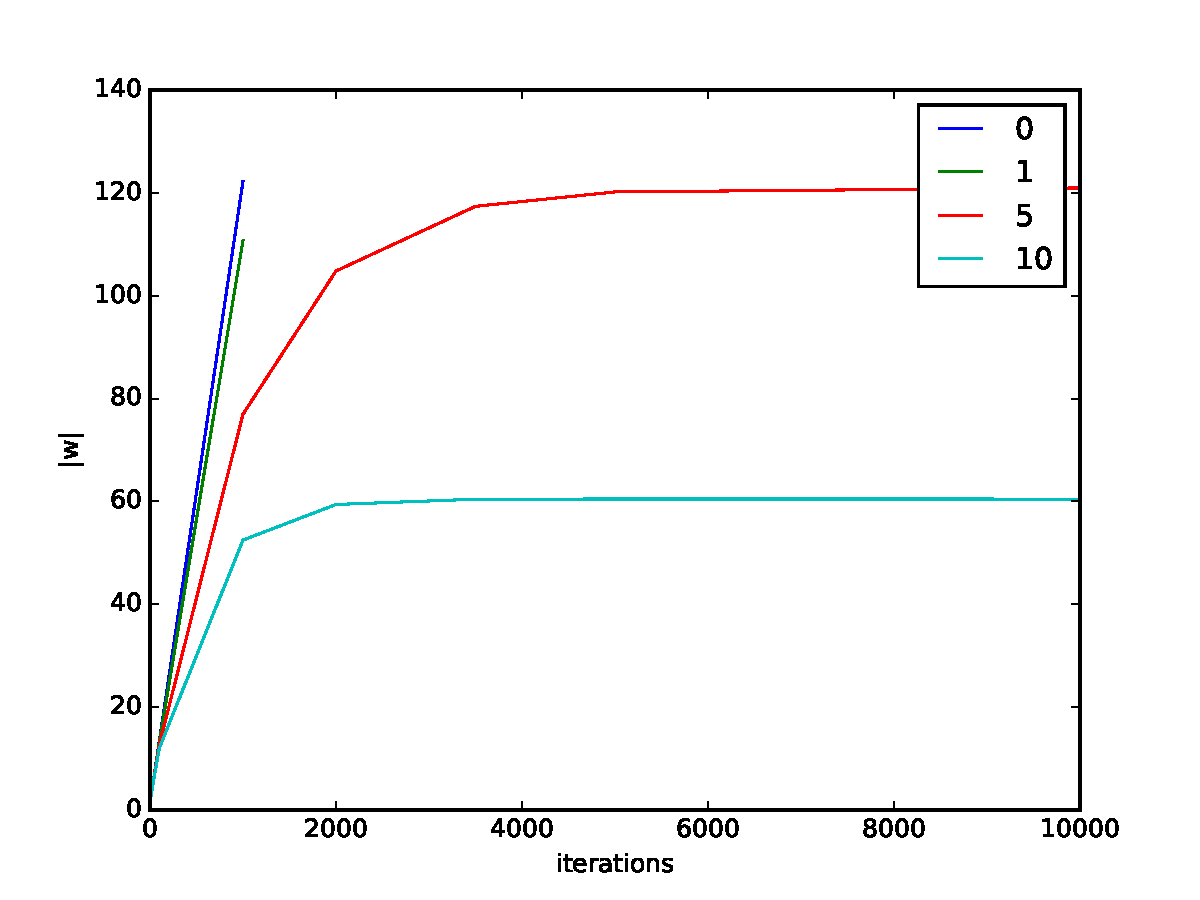
\includegraphics[width=\textwidth]{hw2_1-1_1.pdf}
		\caption{}
	\end{subfigure}
	\begin{subfigure}[b]{0.23\textwidth}
		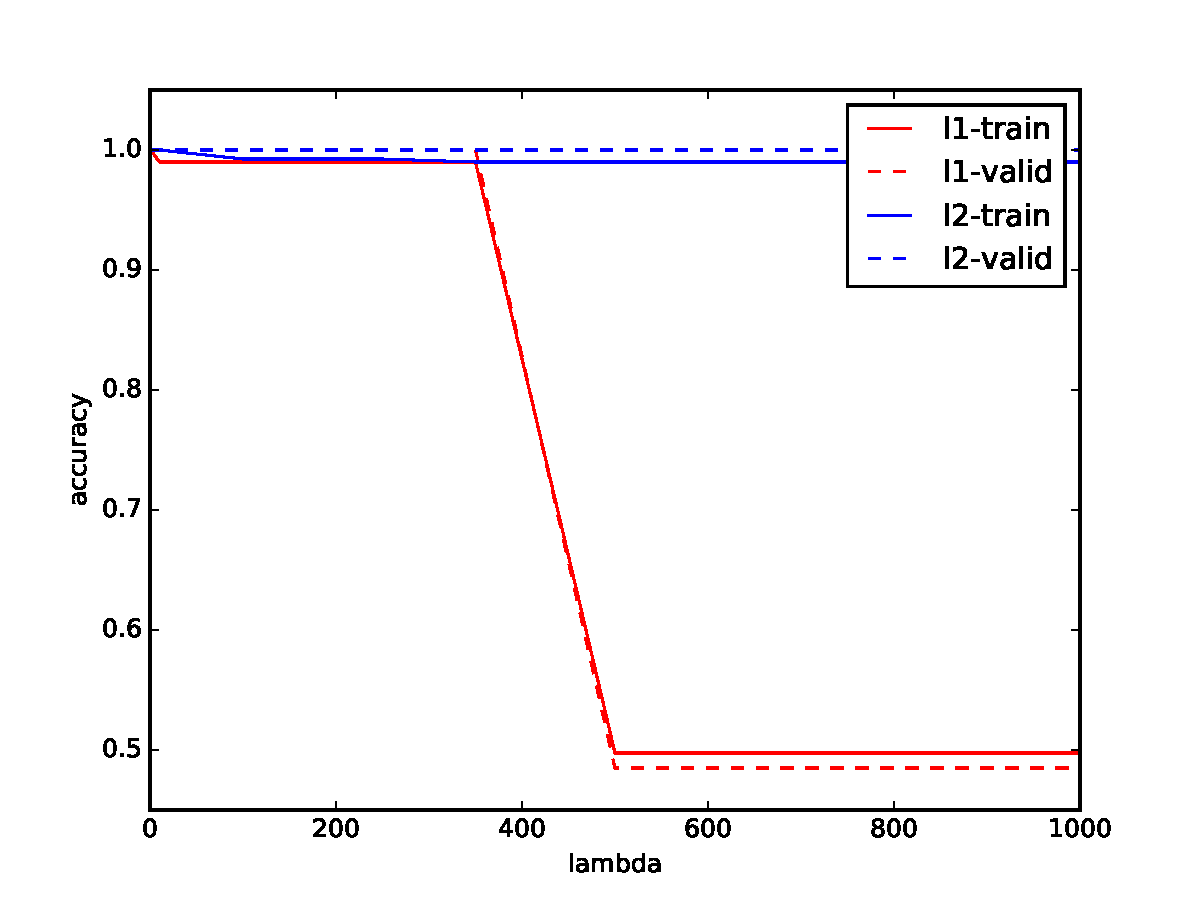
\includegraphics[width=\textwidth]{hw2_1-2_1.pdf}
		\caption{Accuracy}
	\end{subfigure}
	\begin{subfigure}[b]{0.23\textwidth}
		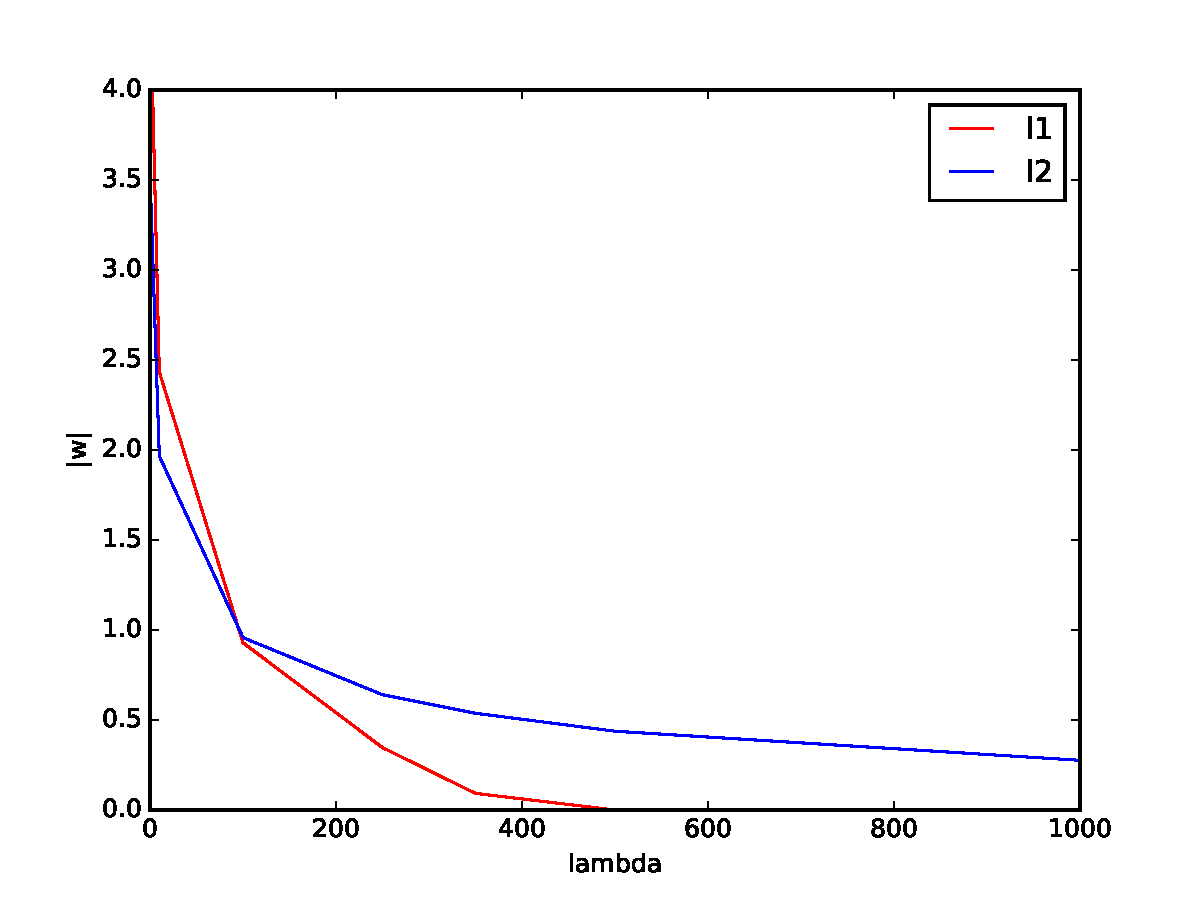
\includegraphics[width=\textwidth]{hw2_1-2_2.pdf}
		\caption{$\|w\|_2$}
	\end{subfigure}
	\begin{subfigure}[b]{0.23\textwidth}
		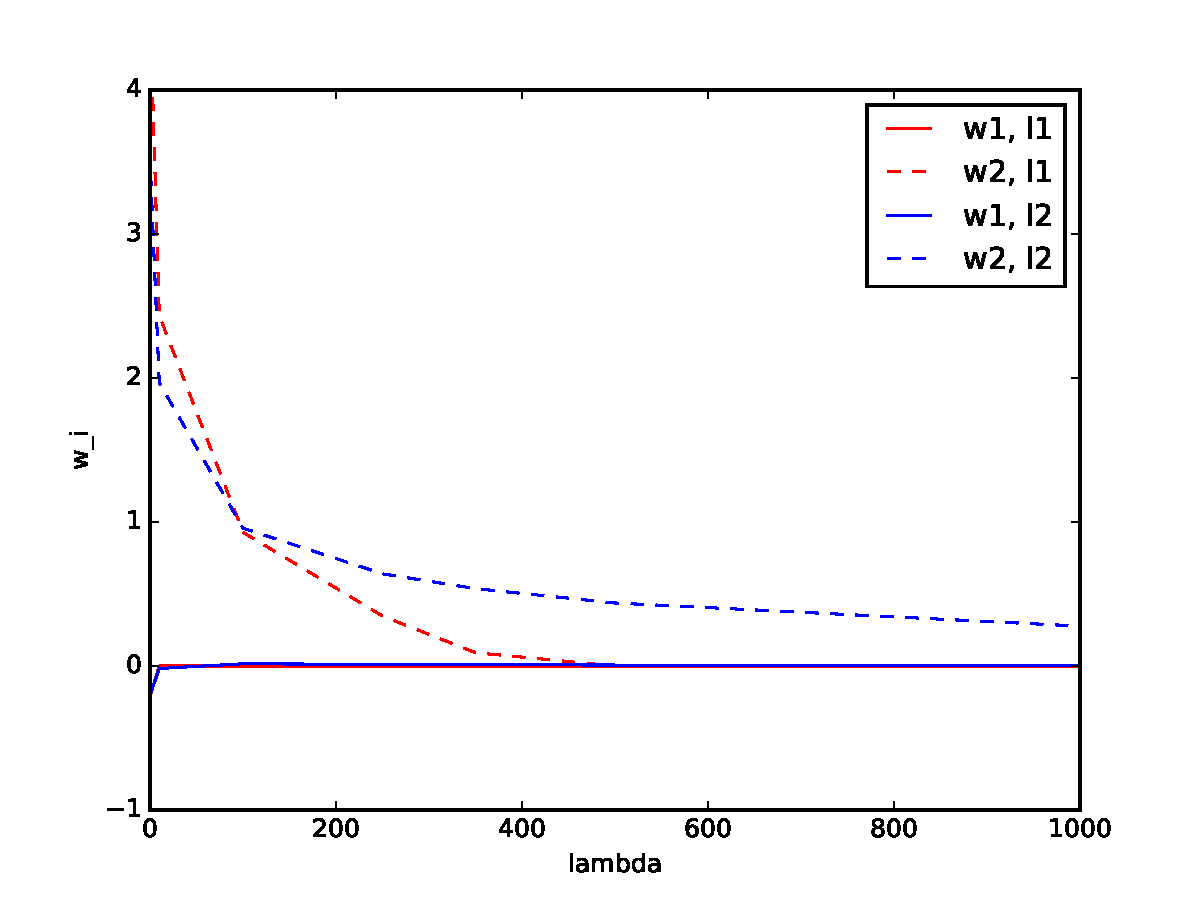
\includegraphics[width=\textwidth]{hw2_1-2_3.pdf}
		\caption{$w_1, w_2$}
	\end{subfigure}
	\caption{Effects of regularization on the weights (coefficients) of logistic regression model for various values of $\lambda$, and under $L_1$ vs. $L_2$ regularization.}
\end{figure}

\begin{figure}
	\centering
	\begin{subfigure}[b]{0.23\textwidth}
		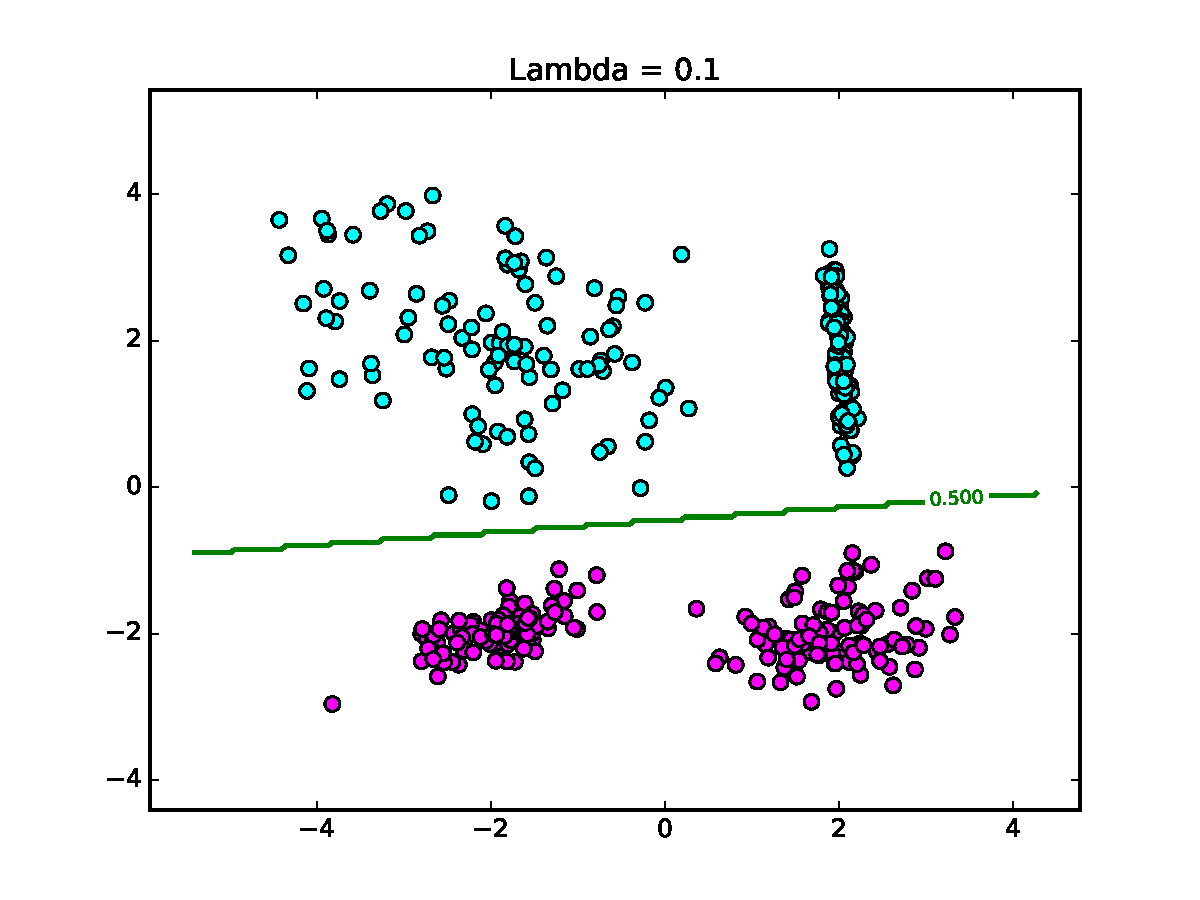
\includegraphics[width=\textwidth]{hw2_1-2_4.pdf}
		\caption{$L_1, \lambda = 0.1$}
	\end{subfigure}
	\begin{subfigure}[b]{0.23\textwidth}
		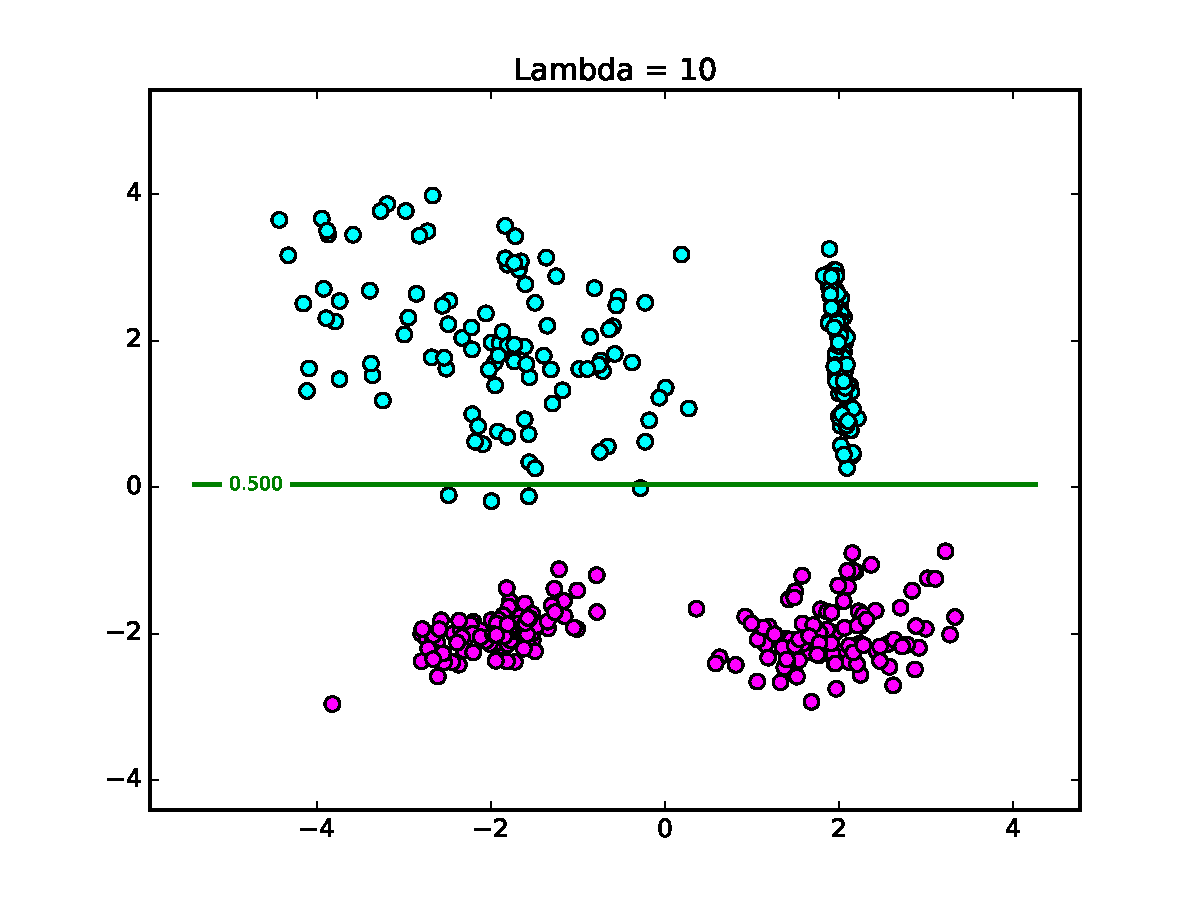
\includegraphics[width=\textwidth]{hw2_1-2_6.pdf}
		\caption{$L_1, \lambda = 10$}
	\end{subfigure}
	\begin{subfigure}[b]{0.23\textwidth}
		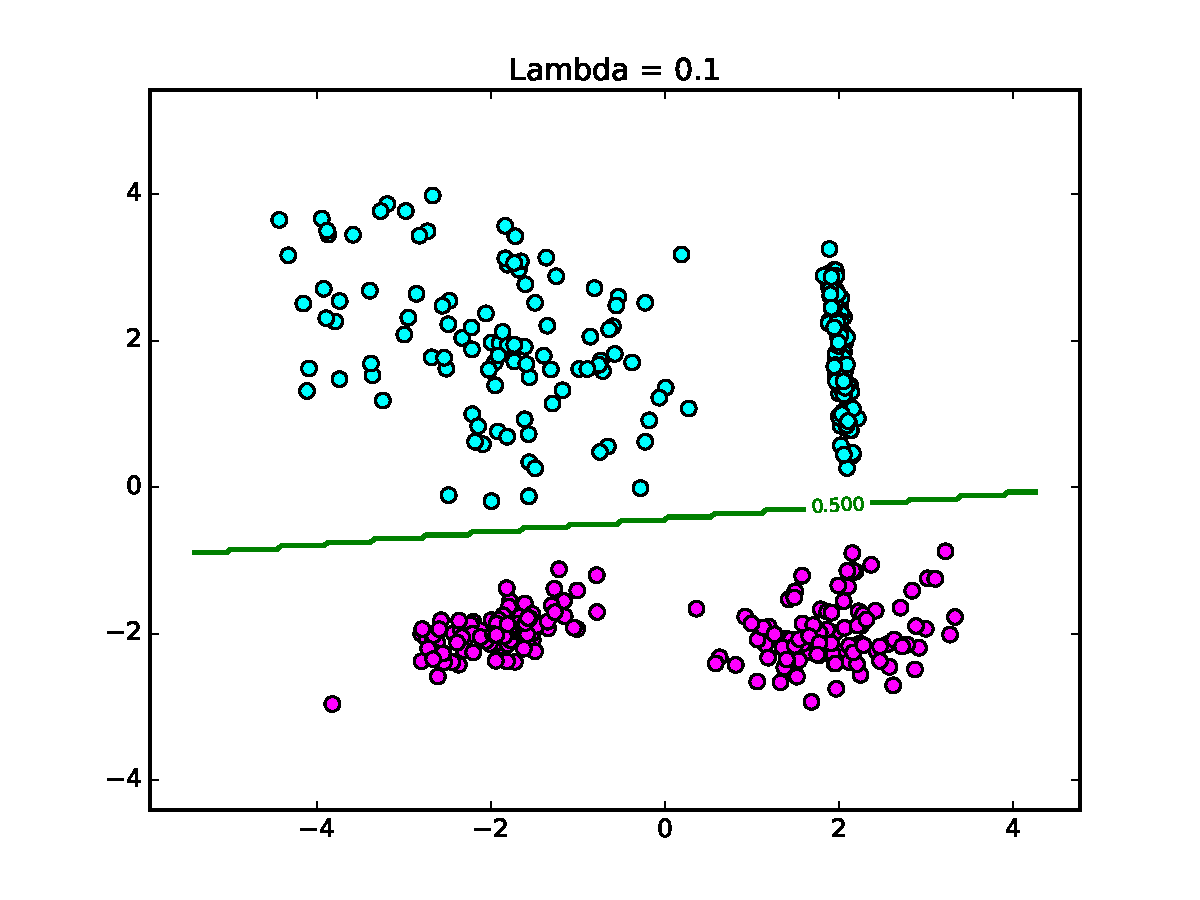
\includegraphics[width=\textwidth]{hw2_1-2_8.pdf}
		\caption{$L_2, \lambda = 0.1$}
	\end{subfigure}
	\begin{subfigure}[b]{0.23\textwidth}
		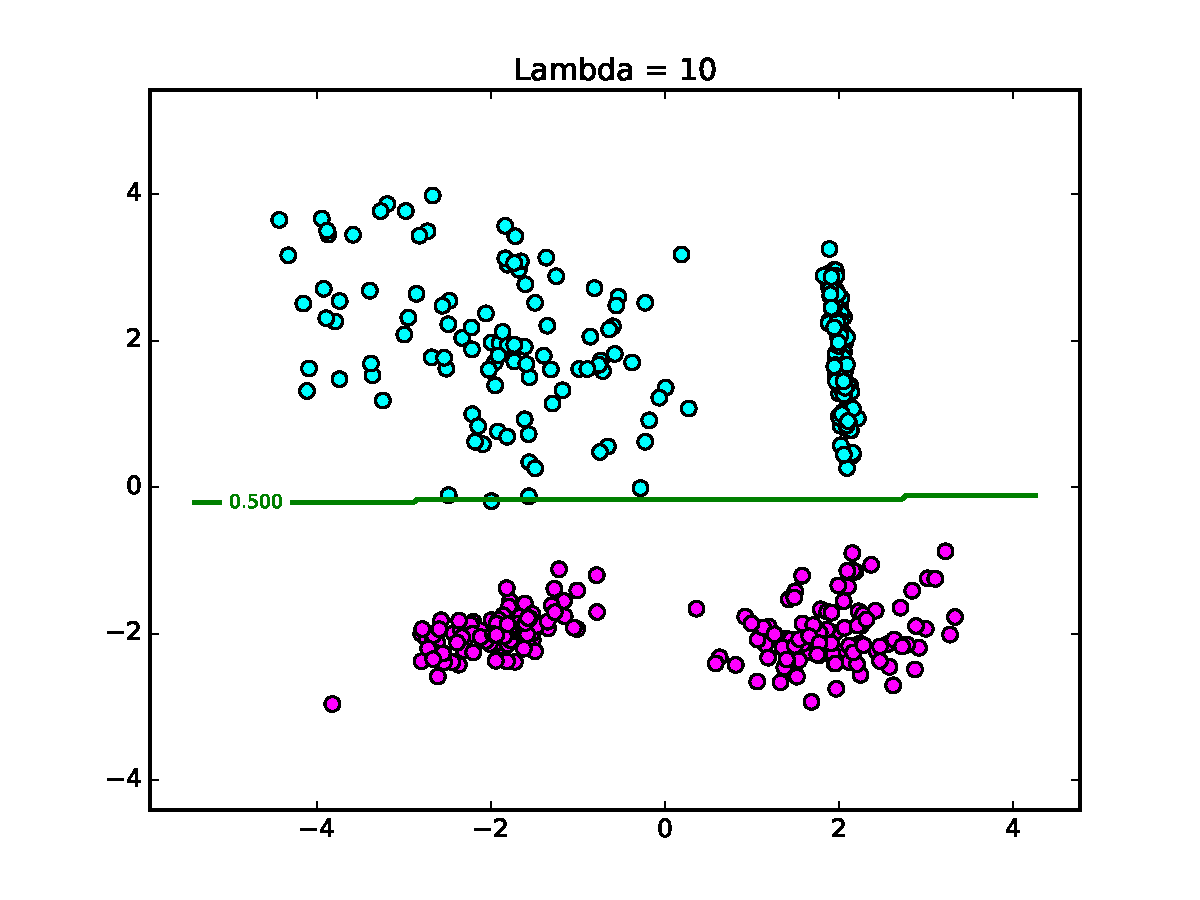
\includegraphics[width=\textwidth]{hw2_1-2_10.pdf}
		\caption{$L_2, \lambda = 10$}
	\end{subfigure}
	\caption{Decision boundaries for the training set for artificial dataset 1, for $L_1$ vs $L_2$ regularization.}
\end{figure}

\begin{figure}
	\centering
	\begin{subfigure}[b]{0.4\textwidth}
		\centering
		\begin{tabular}{c|c|c|c}\hline
			Dataset & Regularizer & $\lambda$ & Accuracy\\\hline
			1 & $L_1$ & 0.01 & 1 \\
			2 & $L_1$ & 0.01 & 0.805\\
			3 & $L_2$ & 0.3& 0.96  \\
			4 & $L_1$ & 100& 0.5 \\\hline
		\end{tabular}
		\caption{Regularizer and $\lambda$ Values}
	\end{subfigure}
	\begin{subfigure}[b]{0.2\textwidth}
		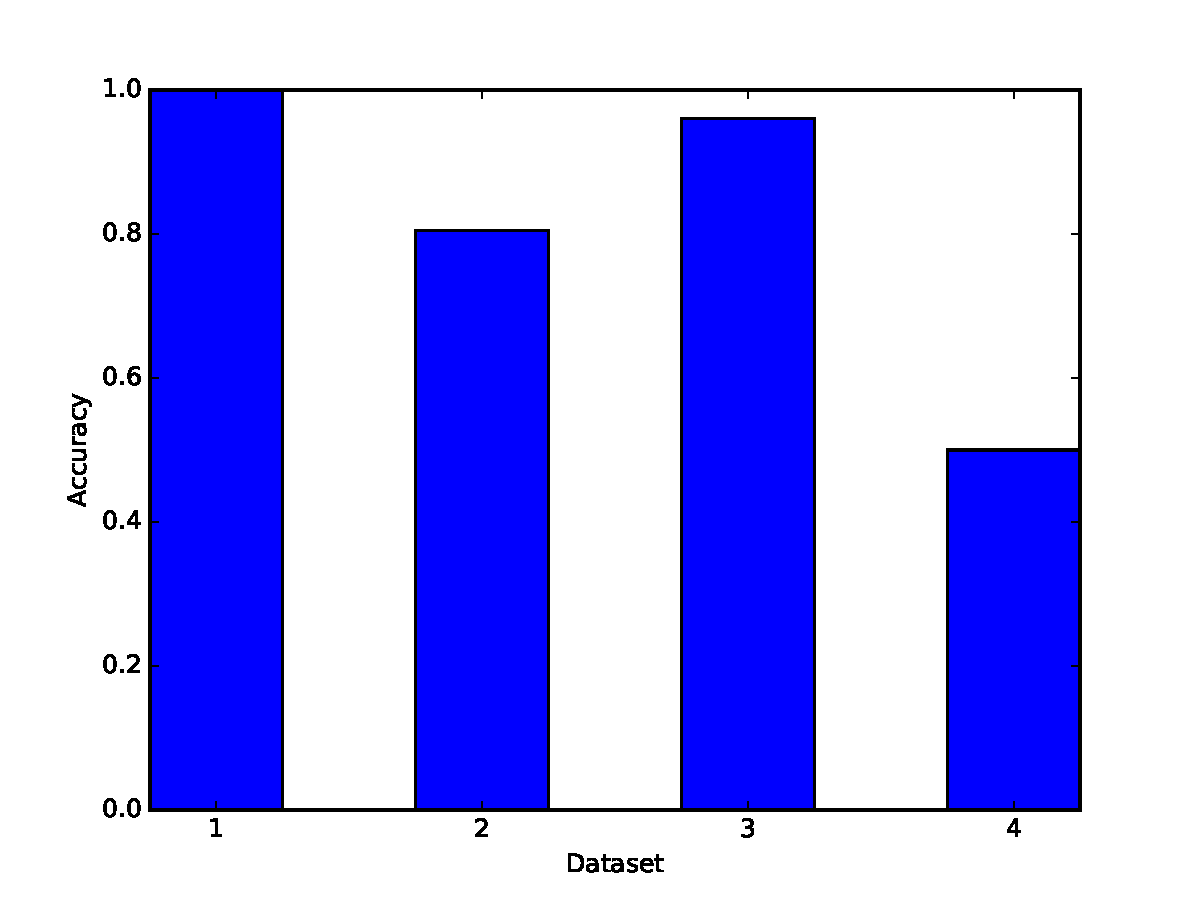
\includegraphics[width=\textwidth]{hw2_1-3_1.pdf}
		\caption{Accuracy}
	\end{subfigure}
	\caption{Best-performing regularizers and $\lambda$ values for each artificial dataset (selected on validation), with classification accuracy on corresponding test set.}
\end{figure}

\section{Support Vector Machine}

Rather than using a discriminative probabilistic model, such as logistic regression, we can also employ a discriminant rule to directly classify points. One example of such a classifier is the support vector machine (SVM), of which the simplest variant is the linear SVM, using no feature transformations. The linear SVM minimizes the following Lagrangian:
$$L(w, b, \xi, a, \mu) = \frac{1}{2}\|w\|^2 + C\sum_n \xi_n - \sum_n a_n(y^n f(x_n) - 1+ \xi_n) - \sum_n \mu_n \xi_n$$
which is equivalent to maximizing the margin while penalizing classification error. Rather than solve this problem directly, however, it is often more convenient to consider the dual Lagrangian for this problem, which is given by:
$$\tilde{L}(a) = \sum_n a_n - \frac{1}{2} \sum_n \sum_m a_na_m y_ny_m K(x_n,x_m) = 1^T a - \frac{1}{2} a^T(YKY)a$$
where we define $a = (a_1, \dots, a_n)$, $Y = diag(y)$, and $1 = (1, \dots, 1)$, with the kernel:
$$K(x,x') = x^Tx'$$
This Lagrangian is then maximized with the constraints $0\leq a_n \leq C$ and $\sum_n a_ny_n = 0$, and can be solved using a standard quadratic programming (QP) algorithm.

\subsection{Implementation Tests} For a simple dataset given in {\bf Figure 4(a)}, we achieve a dual objective value of $-0.154$, and find that the Lagrange multiplier values are (approximately) $ \alpha = (0.154, 0, 0.154, 0)$, so that the support vectors are the first and third examples. {\bf Figure 4(b)} makes this claim appear reasonable, as a hyperplane separating the sets of points would be closest to the first and third examples, as the solutions indicate.

\begin{figure}[h!]
	\centering
\begin{subfigure}[b]{0.15\textwidth}
	\centering
\begin{tabular}{|c|c|c|}\hline
$x_1$ & $x_2$ & $y$ \\\hline
2 & 2 & 1 \\
2 & 3 & 1 \\
0 & -1 & -1\\
-3 & -2 & -1\\\hline
\end{tabular}
\vspace{0.15in}
\caption{}
\end{subfigure}
\begin{subfigure}[b]{0.2\textwidth}
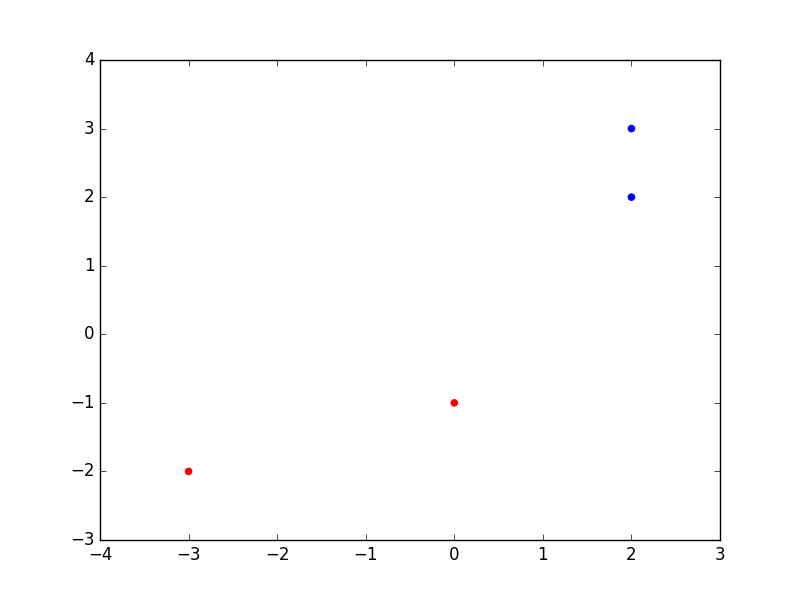
\includegraphics[width=\textwidth]{hw2-2_1-1.png}
\caption{}
\end{subfigure}
\begin{subfigure}[b]{0.2\textwidth}
	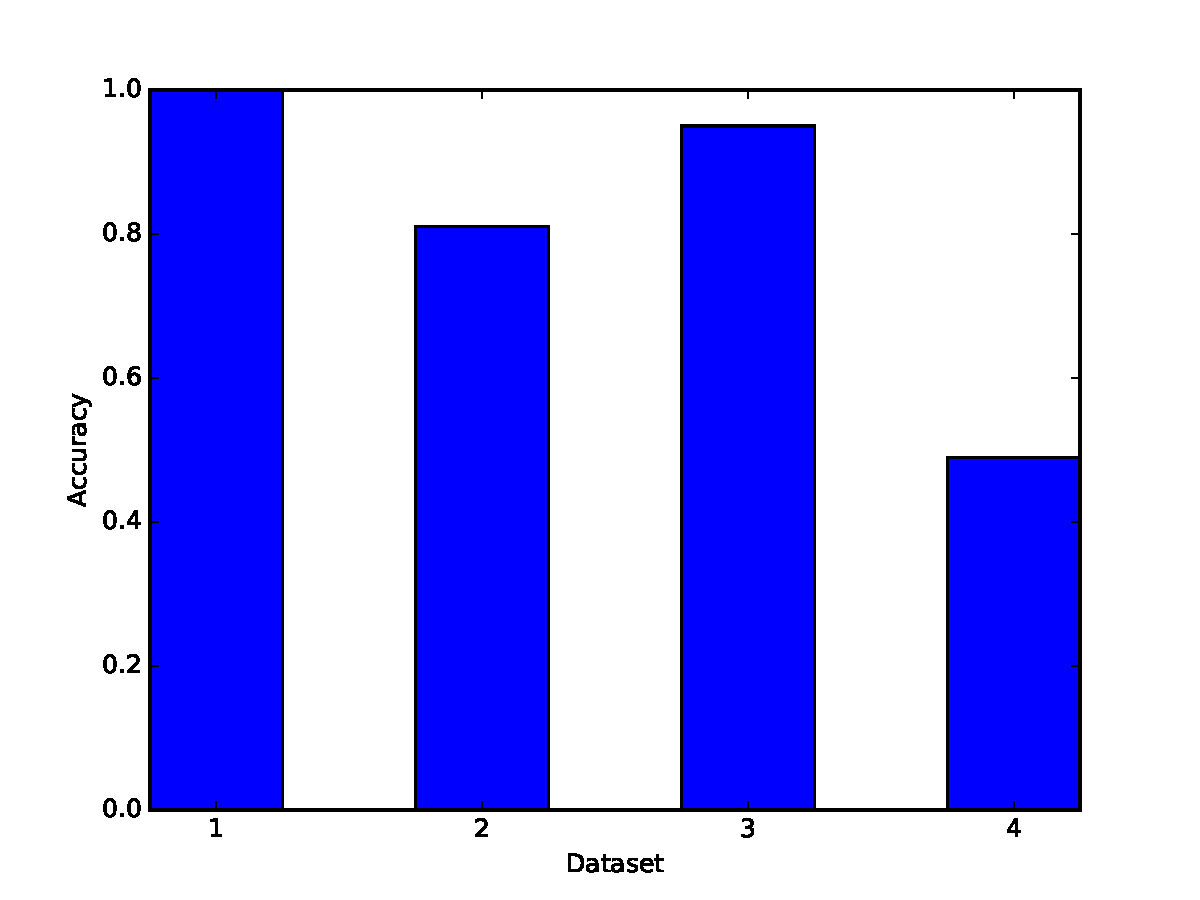
\includegraphics[width=\textwidth]{hw2_2-2_acc.pdf}
	\caption{}
\end{subfigure}
\caption{Simple dataset for testing linear SVM implementation (a, b), and (c) classification accuracy on test set of artificial datasets.}
\end{figure}

\subsection{Comparisons on Artificial Datasets} To explore the differences in classification between the logistic regression, we apply the linear SVM model detailed above to the artificial datasets used in Section 1, using a soft margin parameter of $C = 1$. As in the case of logistic regression, we provide in {\bf Figure 4(c)} the classification accuracy for the linear SVM model on each artificial test dataset, where the model is trained on the respective training set. The plot is very similar to that of {\bf Figure 3(b)}, which is the corresponding classification accuracies achieved by fine-tuned logistic regression classifiers, despite no hyperparameter selection (for $C$) for the linear SVM classifiers.

Moreover, {\bf Figure 5} depicts the resulting decision boundaries for the training set of each artificial dataset, which provides further evidence on the correctness of the implementation, as the boundaries appear reasonable in separating the classes when the data is linearly separable. A comparison between {\bf Figure 5(a)} and {\bf Figure 2} suggests that compared to the logistic regression model, the linear SVM does in fact learn a higher-margin classifer than logistic regression with either regularization. It is interesting to note that this higher-margin property does indeed yield a visually ``cleaner'' boundary, which holds for the other datasets as well (not displayed here for space considerations).

\begin{figure}
	\centering
	\begin{subfigure}[b]{0.23\textwidth}
		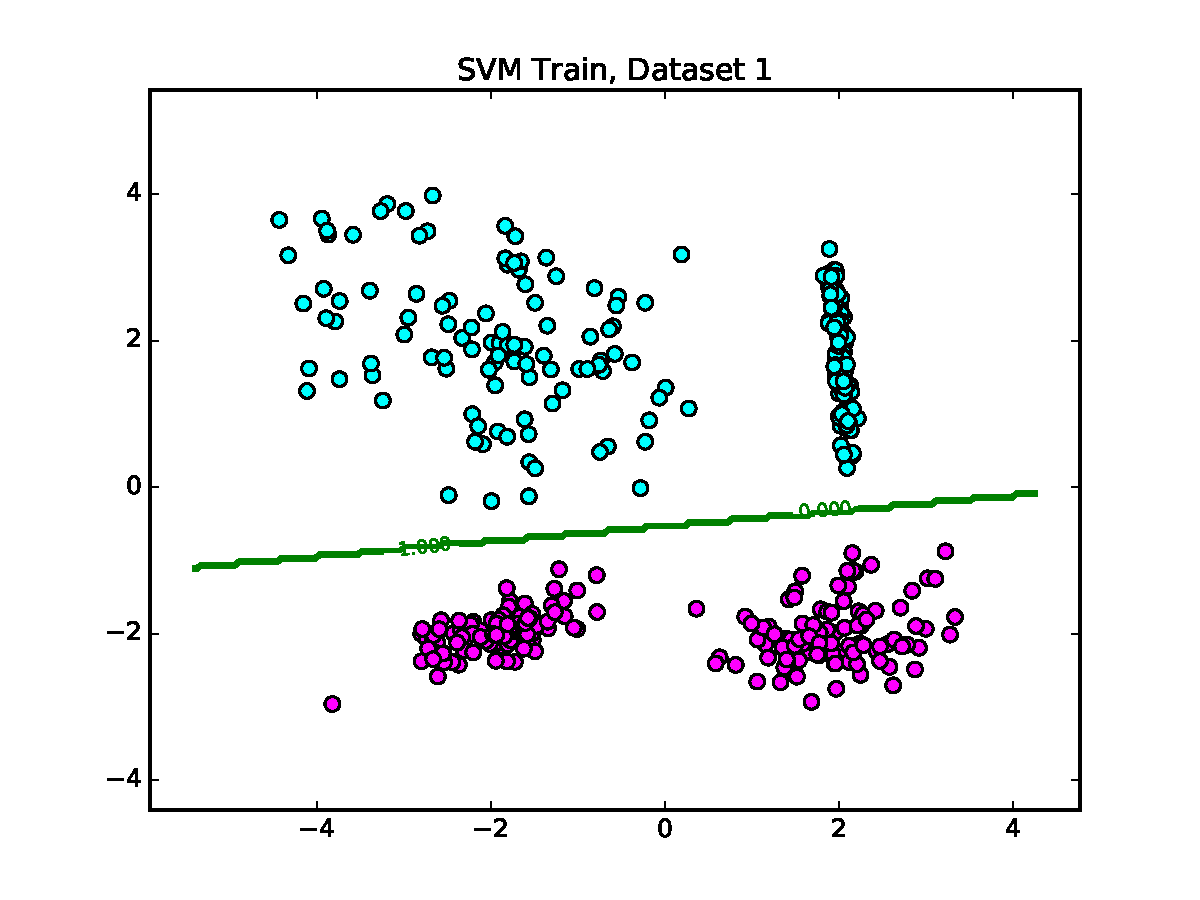
\includegraphics[width=\textwidth]{hw2_2-2_1_train.pdf}
		\caption{Dataset 1}
	\end{subfigure}
	\begin{subfigure}[b]{0.23\textwidth}
		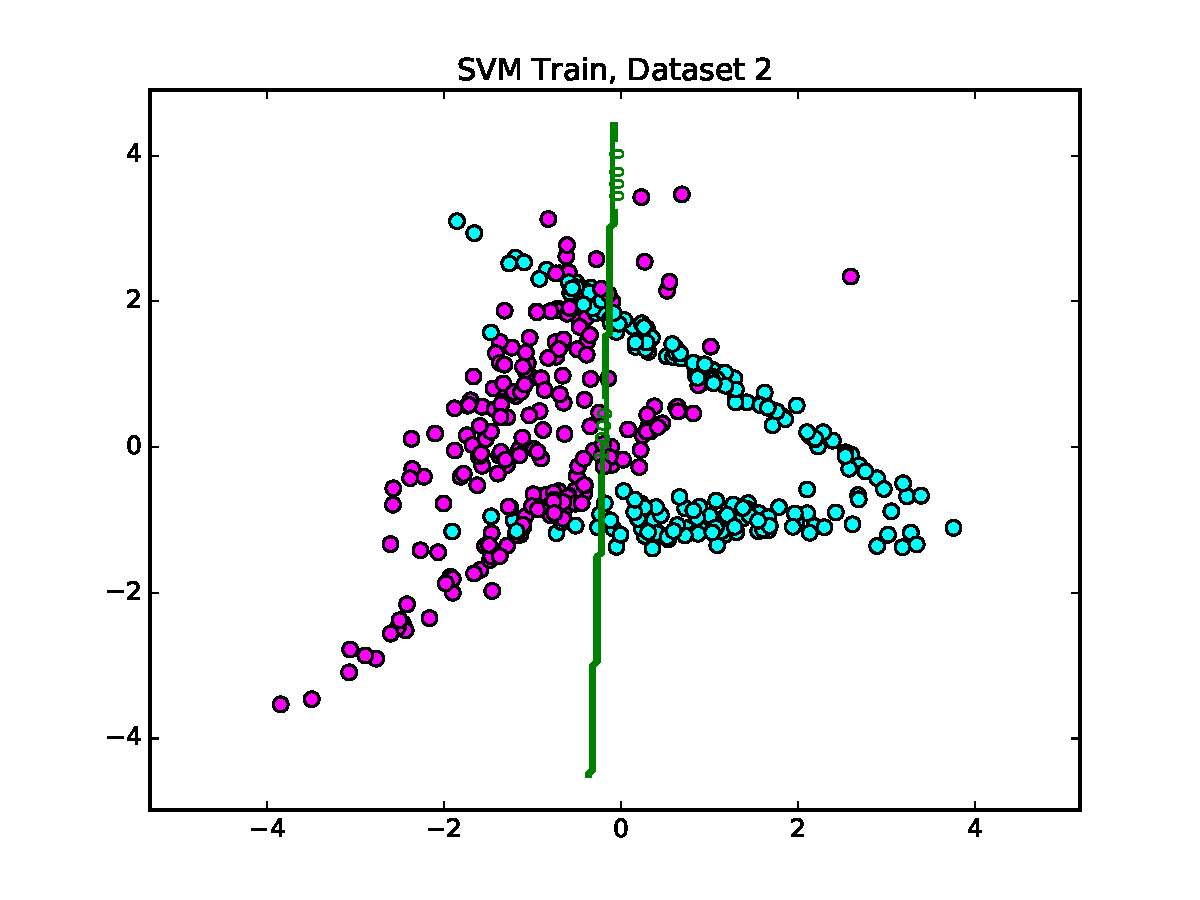
\includegraphics[width=\textwidth]{hw2_2-2_2_train.pdf}
		\caption{Dataset 2}
	\end{subfigure}
	\begin{subfigure}[b]{0.23\textwidth}
		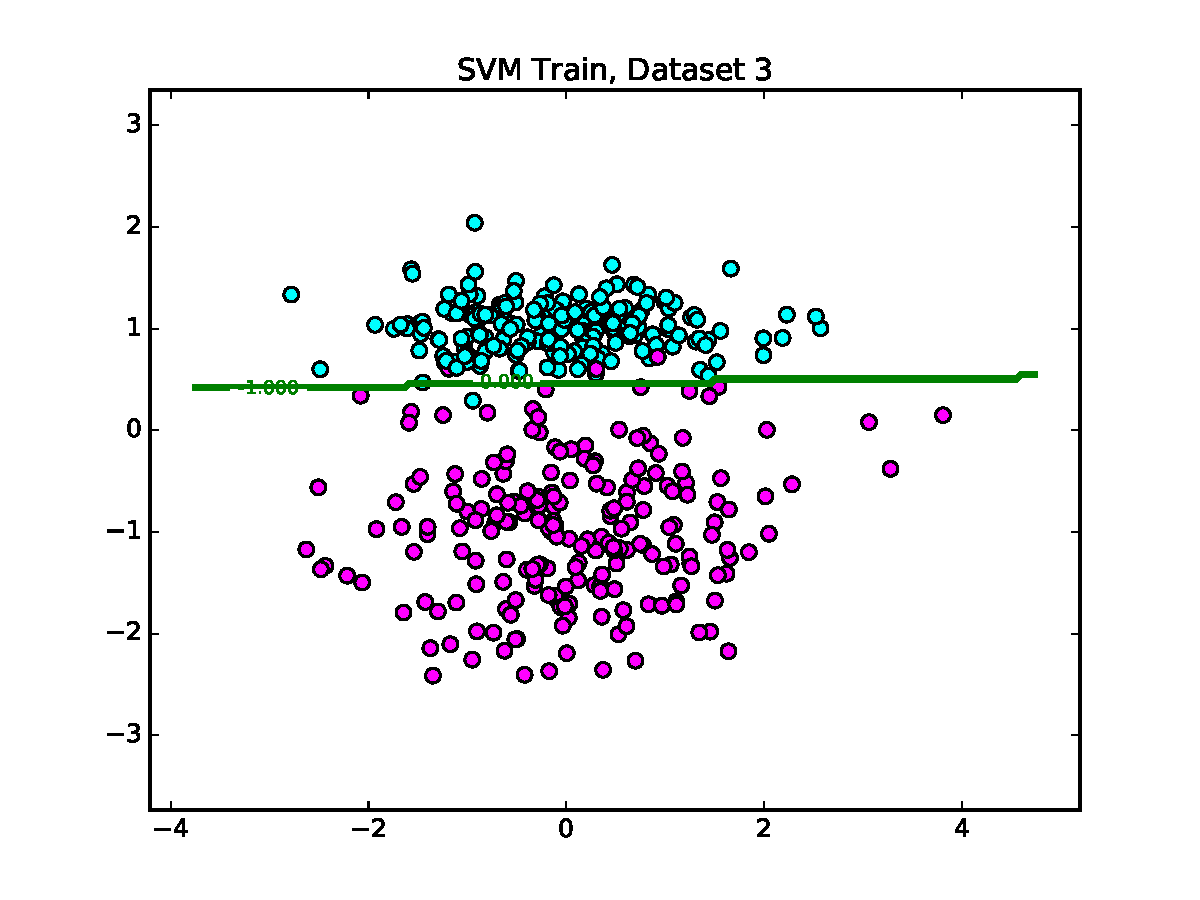
\includegraphics[width=\textwidth]{hw2_2-2_3_train.pdf}
		\caption{Dataset 3}
	\end{subfigure}
	\begin{subfigure}[b]{0.23\textwidth}
		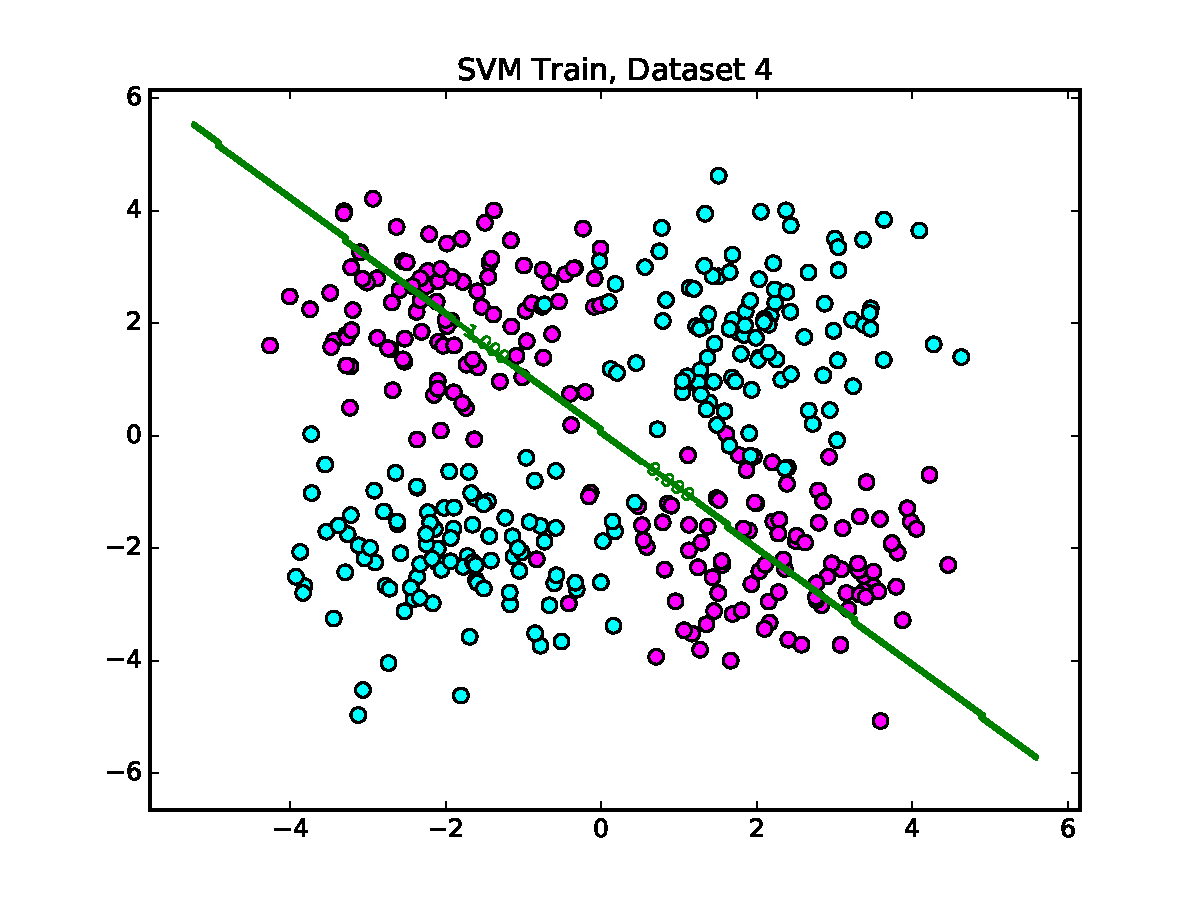
\includegraphics[width=\textwidth]{hw2_2-2_4_train.pdf}
		\caption{Dataset 4}
	\end{subfigure}
	\caption{Decision boundaries for the training set for artificial datasets 1 through 4, using linear SVM with $C = 1$.}
\end{figure}

\subsection{Hyperparameters for Linear and Gaussian RBF Kernels} We now investigate the dependence of the solutions found by the SVM depend on the hyperparameters of the classifier. We employ the kernelized dual SVM with the Lagrangian $\tilde{L}(a)$ provided above, with two different kernels: 1) the linear kernel $K(x,x') = x^Tx$ as employed above, and 2) the Gaussian radial basis function (RBF) kernel $K(x,x') = \exp(-\gamma \|x-x'\|^2)$. Thus, we vary the hyperparameter $C = 10^{-2}, 10^{-1}, \dots, 10^2$ for both kernel models, and for the Gaussian kernel we also vary the kernel bandwidth $\gamma = 10^{-3}, 10^{-2}, \dots, 10^2$.

Our results are demonstrated in {\bf Figure 6}, where we have displayed the hyperparameters on the logarithmic scale for illustration. We see that for the linear kernel, a increase in the slack penalty $C$ yields a smaller margin size as well as decrease in the number of support vectors. This makes intuitive sense, since increasing $C$ leads to less penalization of the $L_2$ norm of the weights, which leads to larger $\|w\|^2$ and thus smaller margins $1/\|w\|$. With smaller margins, we will tend to have fewer points inside or on the margin since it is a linear hyperplane, so the number of support vectors correspondingly decreases with $C$ as well.

For the Gaussian kernel, we again see that increasing $C$ while keeping $\gamma$ fixed yields a smaller margin size as expected. However, there are more complex dependencies because of the nonlinearity of the kernel as well as the dependence on an additional hyperparameter ($\gamma$). Indeed, we note that it is not necessarily the case that the number of support vectors declines as $C$ increases, and there is also no consistent trend in the dependence of margins or support vectors on $\gamma$. In general, margin sizes appear to decrease with $\gamma$ for a fixed $C$, while the number of support vectors increases with $\gamma$. This last observation is explained by the fact that a larger $\gamma$ corresponds to less influence of each point on the predictor, so that more support vectors are needed to make an accurate prediction. However, note that for the Gaussian kernel, these relationships are not necessarily monotone; for certain values of $C$, increasing $\gamma$ may yield a temporary decline in the number of support vectors, despite the overall tendency.

\begin{figure}[b]
	\centering
	\begin{subfigure}[b]{0.23\textwidth}
		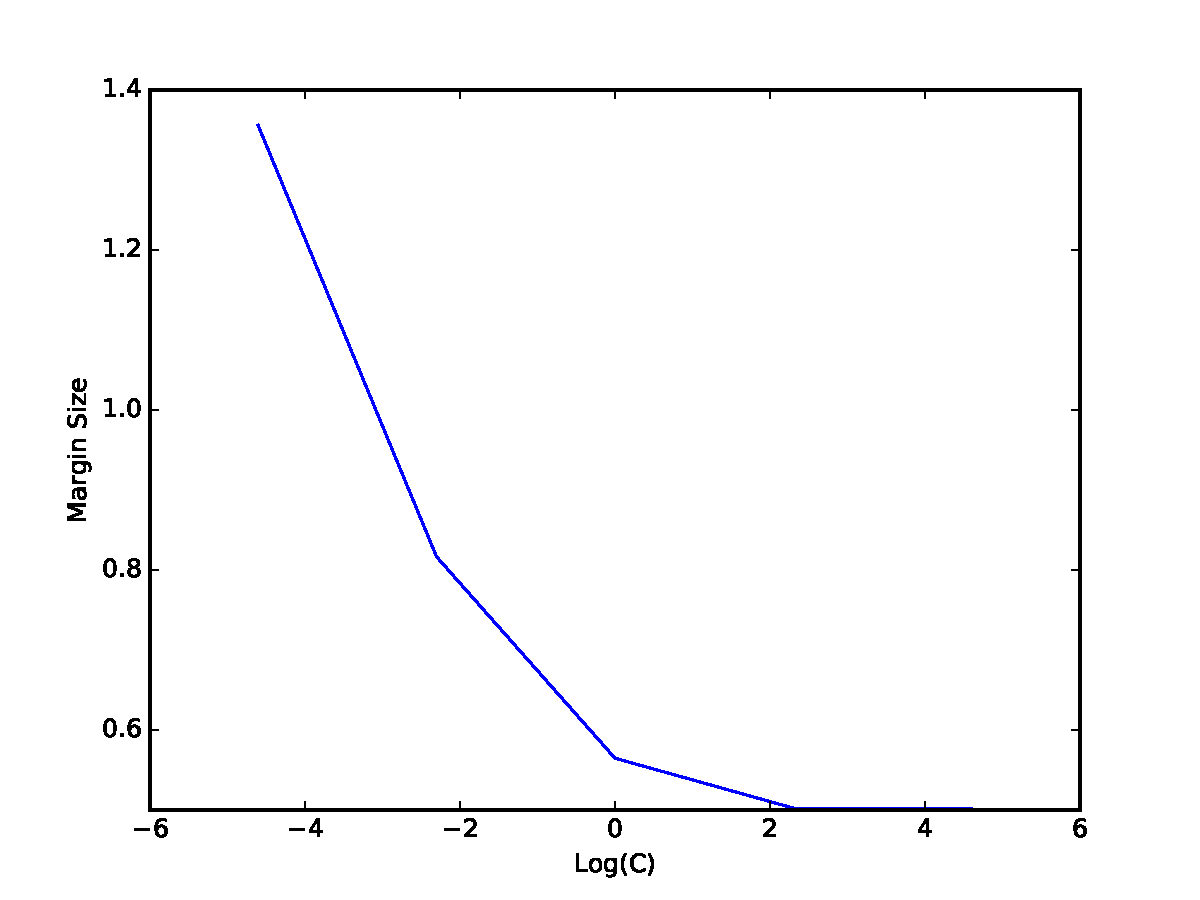
\includegraphics[width=\textwidth]{hw2-2_3_linmargins.pdf}
		\caption{Margin Sizes, Linear Kernel}
	\end{subfigure}
	\begin{subfigure}[b]{0.23\textwidth}
		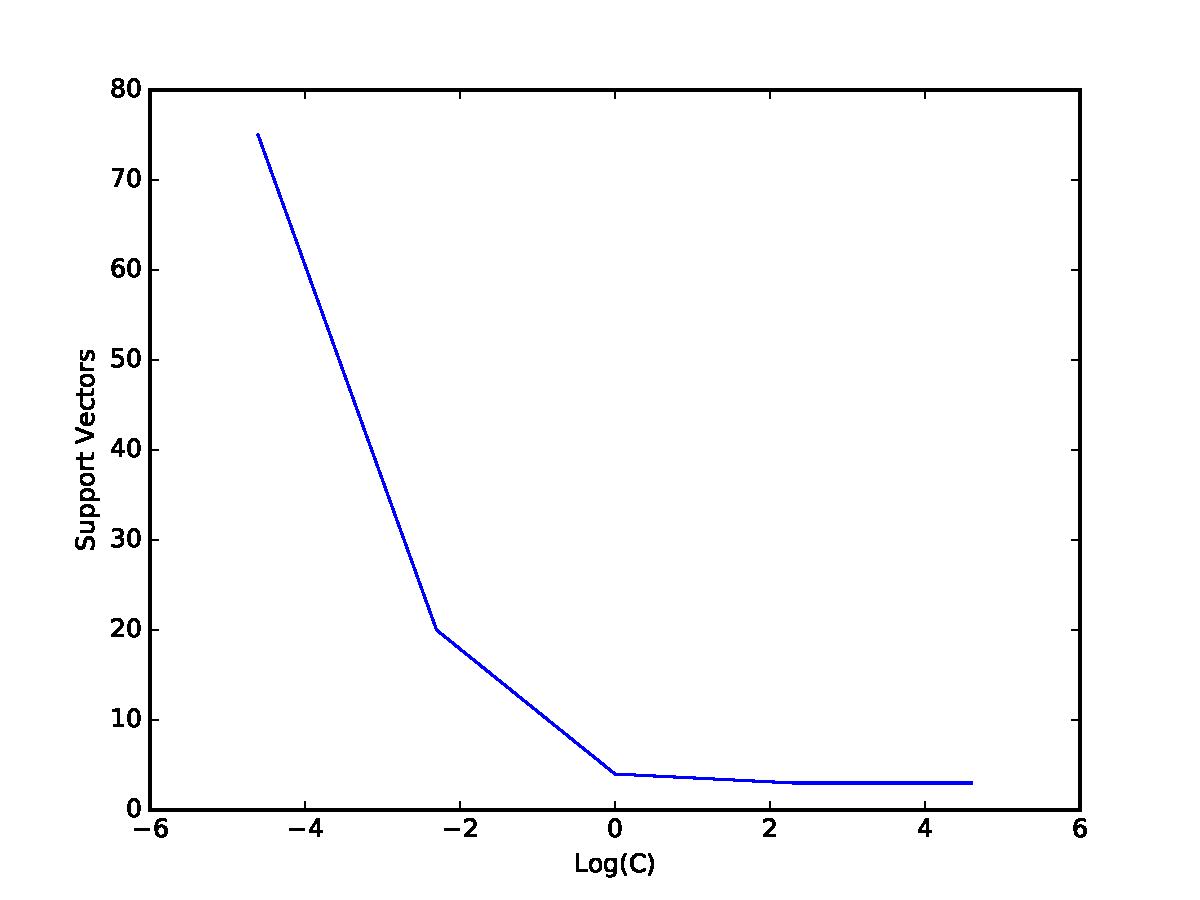
\includegraphics[width=\textwidth]{hw2-2_3_linsv.pdf}
		\caption{Support Vectors, Linear Kernel}
	\end{subfigure}
	\begin{subfigure}[b]{0.23\textwidth}
		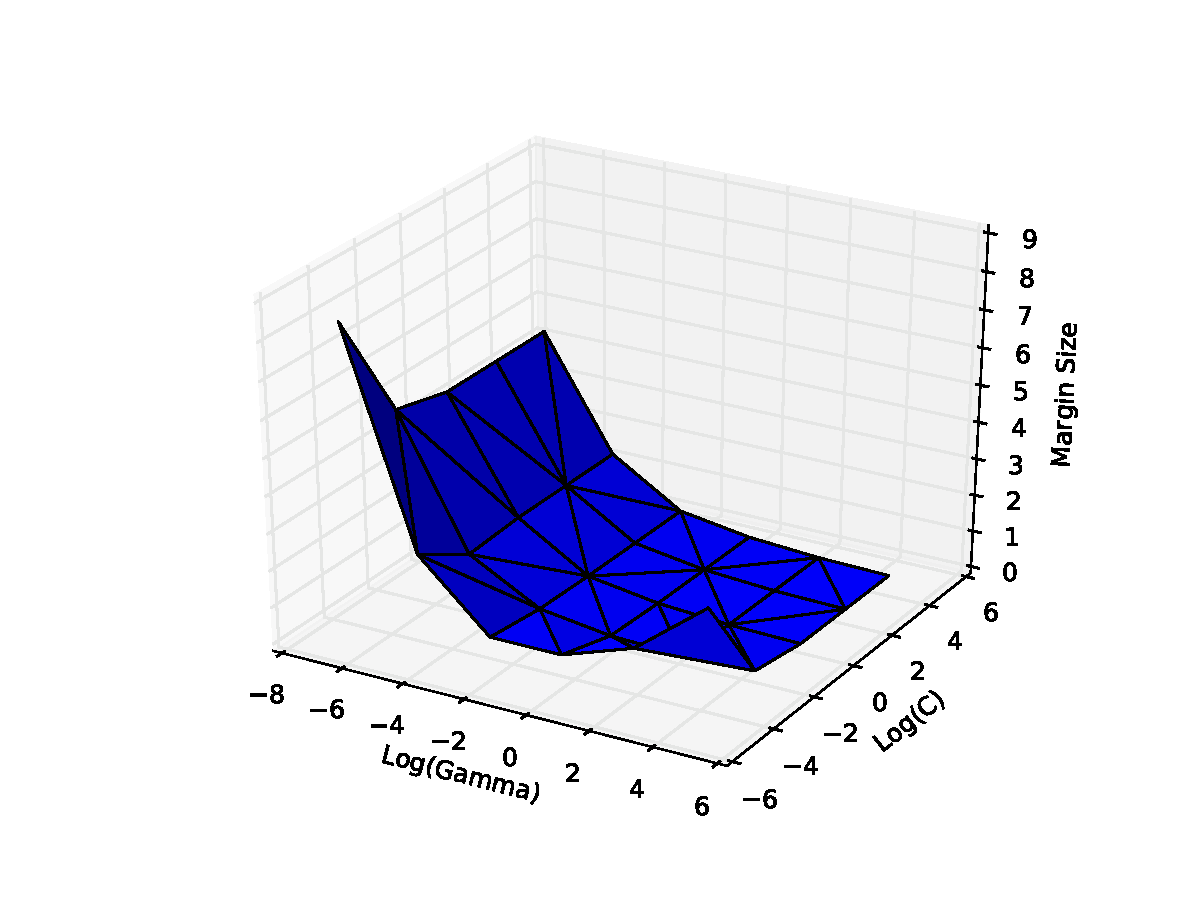
\includegraphics[width=\textwidth]{hw2-2_3_gausmargins.pdf}
		\caption{Margin Sizes, Gaussian Kernel}
	\end{subfigure}
	\begin{subfigure}[b]{0.23\textwidth}
		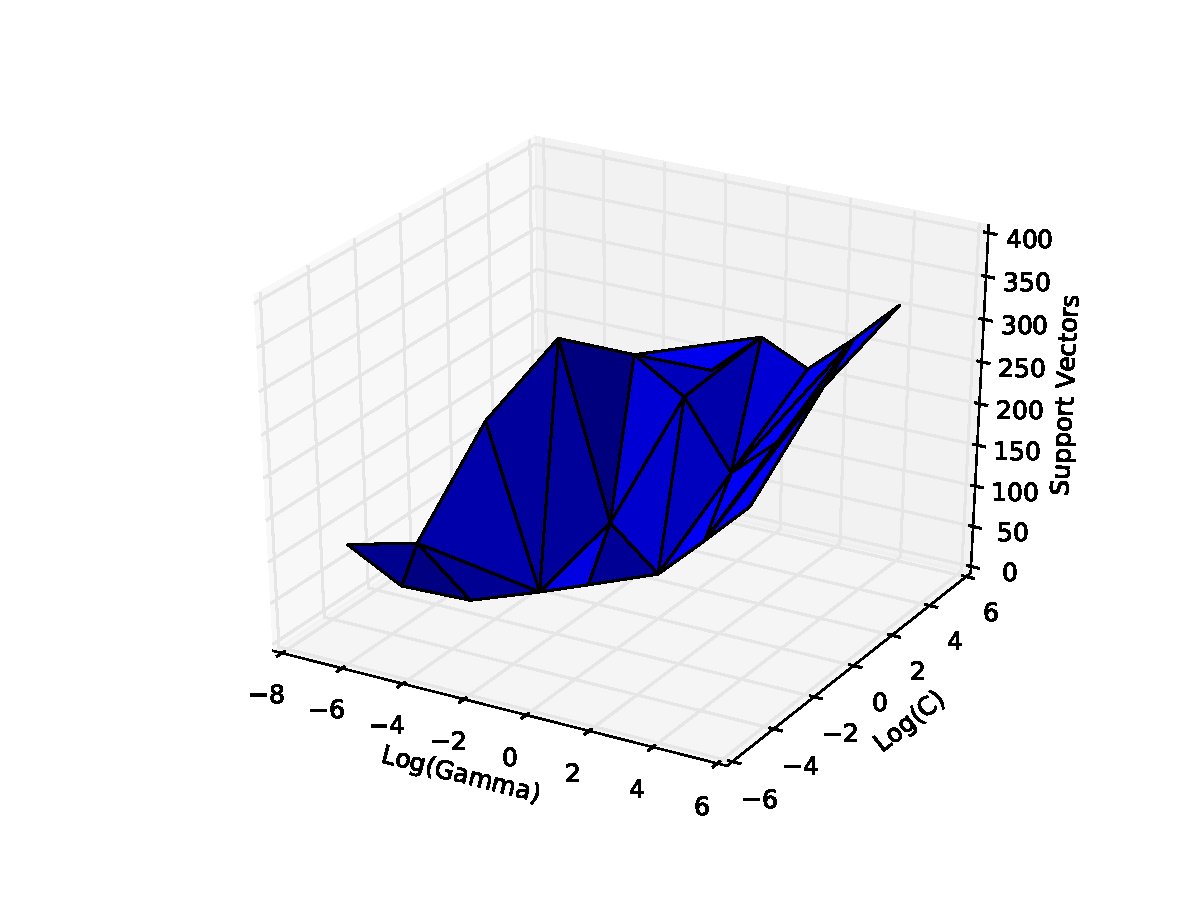
\includegraphics[width=\textwidth]{hw2-2_3_gaussv.pdf}
		\caption{Support Vectors, Gaussian Kernel}
	\end{subfigure}
	\caption{Margin sizes and number of support vectors for varying $C$ (for linear kernels) as well as $\gamma$ (for Gaussian kernels).}
\end{figure}


\section{Support Vector Machine with Pegasos}

An equivalent formulation of the linear SVM with slack constraints (C-SVM) employed in Section 2 is the Soft-SVM using hinge loss. That is, the objective of the C-SVM:
$$\min_w C \sum_n \xi_n+ \frac{1}{2}\|w\|^2$$
can equivalently be written in terms of the hinge loss as:
$$\min_w \frac{\lambda}{2} \|w\|^2  + \sum_n [1-y_n(w^Tx_n)]_+$$
which automatically incorporates the slack constraints as part of the objective. This objective function can then be minimized using the Pegasos algorithm to yield direct solutions $\hat{w}$. In order to compare the results obtained by Pegasos to standard dual formulations of the C-SVM, we begin by exploring the dependence of the algorithm on $\lambda$ and hyperparameters of the basis functions, as in the previous sections. For all experiments, we fix the maximum number of epochs (of training) at $20 \cdot N$, where $N$ is the size of the data, as recommended by Sontag et al.\footnote{http://cs.nyu.edu/~dsontag/courses/ml16/slides/lecture5.pdf}

\subsection{Dependence on $\lambda$} We first consider the regularization parameter $\lambda$ by investigating the dependence of the weights $w$ and the corresponding margin sizes $1/\|w\|$ on the regularization. From the objective function given for the Soft-SVM, it is expected that as $\lambda$ increases, we penalize small margins (large $\|w\|$) more strongly than achieving low classification error, and so our margin sizes should rise at the cost of potentially more misclassified points in the training set.

{\bf Figure 7} demonstrates this behavior, where we used artificial dataset 3 for illustrative purposes. As suspected, increasing the regularization strength $\lambda$ yields a larger-margin classifier, but with higher (at least nondecreasing) numbers of misclassified points. In {\bf Figure 7(a)}, we see that the margin size $1/\|w\|$ does in fact tend to rise with the regularization strength. Interestingly, however, the $\lambda = 1$ yields a decline in margin size, which appears to suggest an issue in the optimization during cases with high regularization; note that with the equivalence of $C = 1/n\lambda$, we see that $\lambda = 1$ in this case would correspond to $C = 1/n$, which is an extreme value that can yield numerical instability.

On the other hand, {\bf Figures 7(b)-(d)} illustrate the fact that as $\lambda$ increases, more and more points end up on the wrong side of the decision boundary, as classification accuracy is sacrificed for larger margin sizes. Indeed, for $\lambda = 2^{-10}$, the decision boundary and classification of points is indistinguishable from the boundary given for the C-SVM in {\bf Figure 5(c)}, and this behavior persists for low $\lambda$ values (i.e. $\lambda \leq 2^{-8}$). As $\lambda$ increases however, the boundary becomes steeper due to penalization of the magnitude of $w_2$, which thereby becomes lower and the normal vector becomes more horizontal. This leads to more negative points being classified as positive points above the boundary. At the other extreme of $\lambda = 1$, we see that nearly half of the negative points have been classified as positive, and the classifier learns very little compared to chance.

\begin{figure}
	\centering
	\begin{subfigure}[b]{0.23\textwidth}
		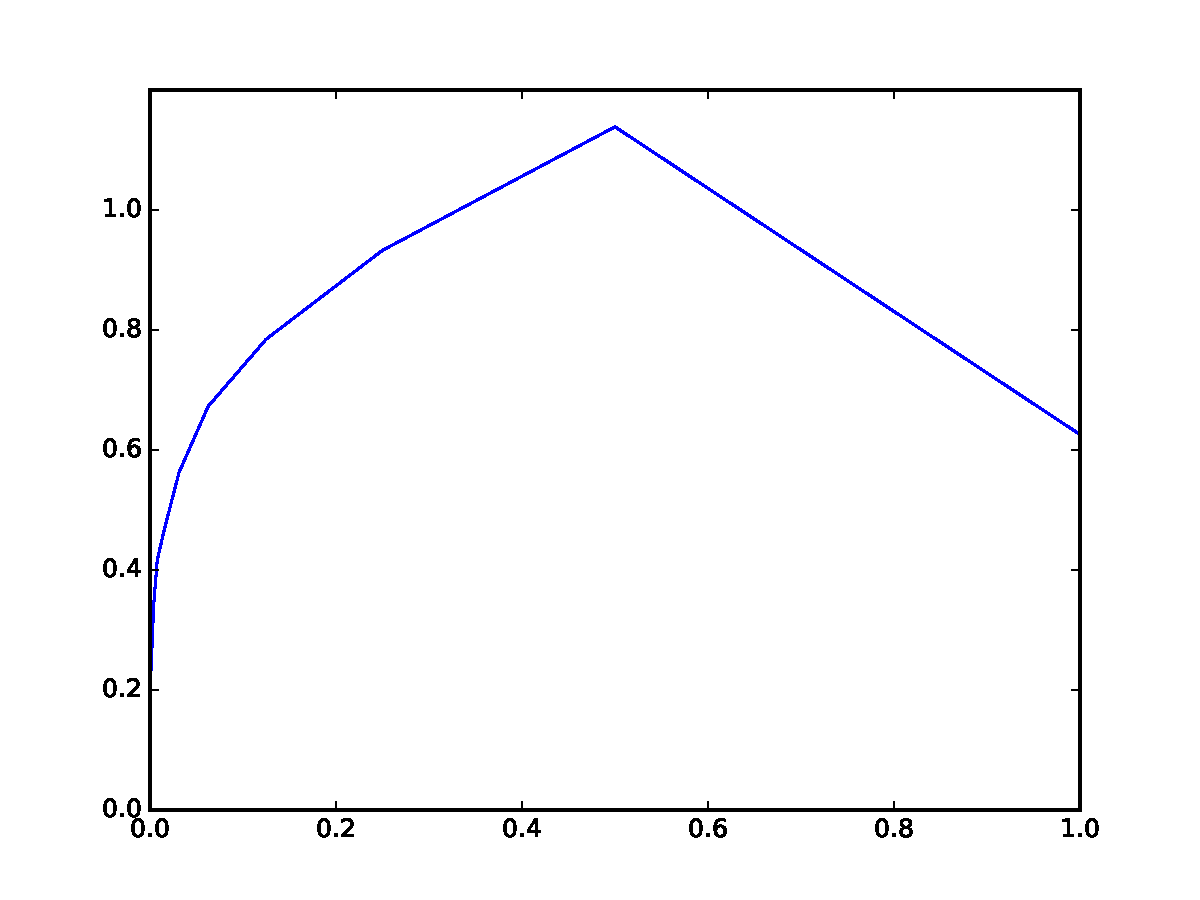
\includegraphics[width=\textwidth]{hw2_3-2_margins.pdf}
		\caption{Margin sizes}
	\end{subfigure}
	\begin{subfigure}[b]{0.23\textwidth}
		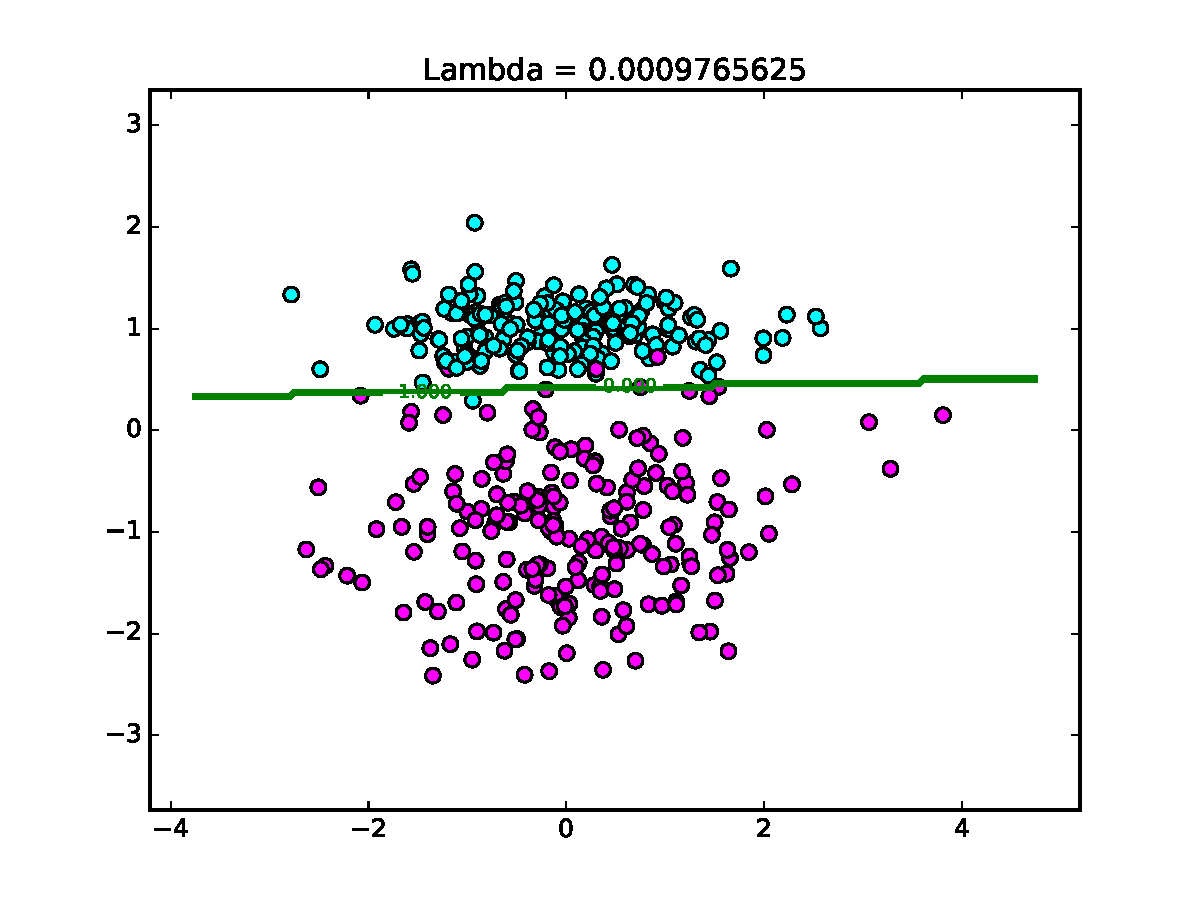
\includegraphics[width=\textwidth]{hw2_3-2_11.pdf}
		\caption{$\lambda = 2^{-10}$}
	\end{subfigure}
	\begin{subfigure}[b]{0.23\textwidth}
		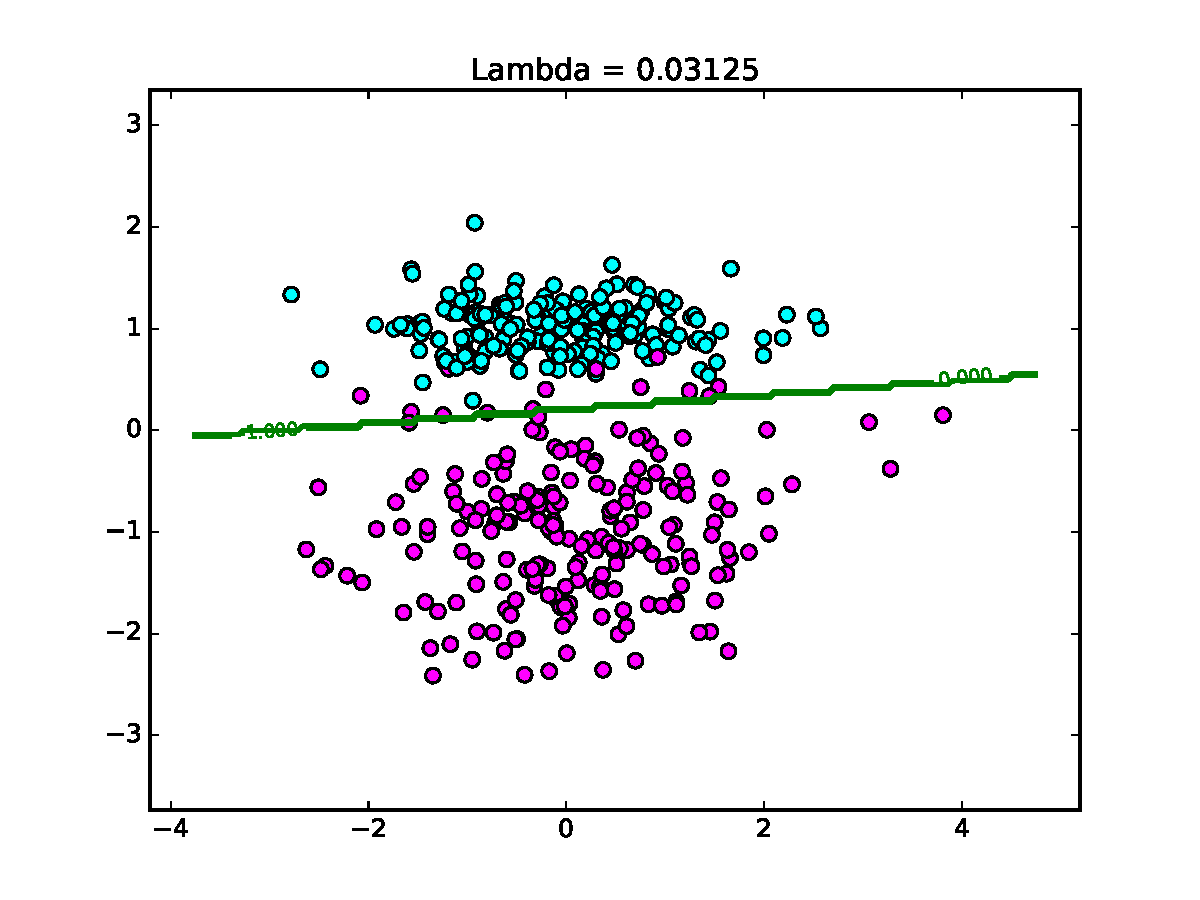
\includegraphics[width=\textwidth]{hw2_3-2_6.pdf}
		\caption{$\lambda = 2^{-5}$}
	\end{subfigure}
	\begin{subfigure}[b]{0.23\textwidth}
		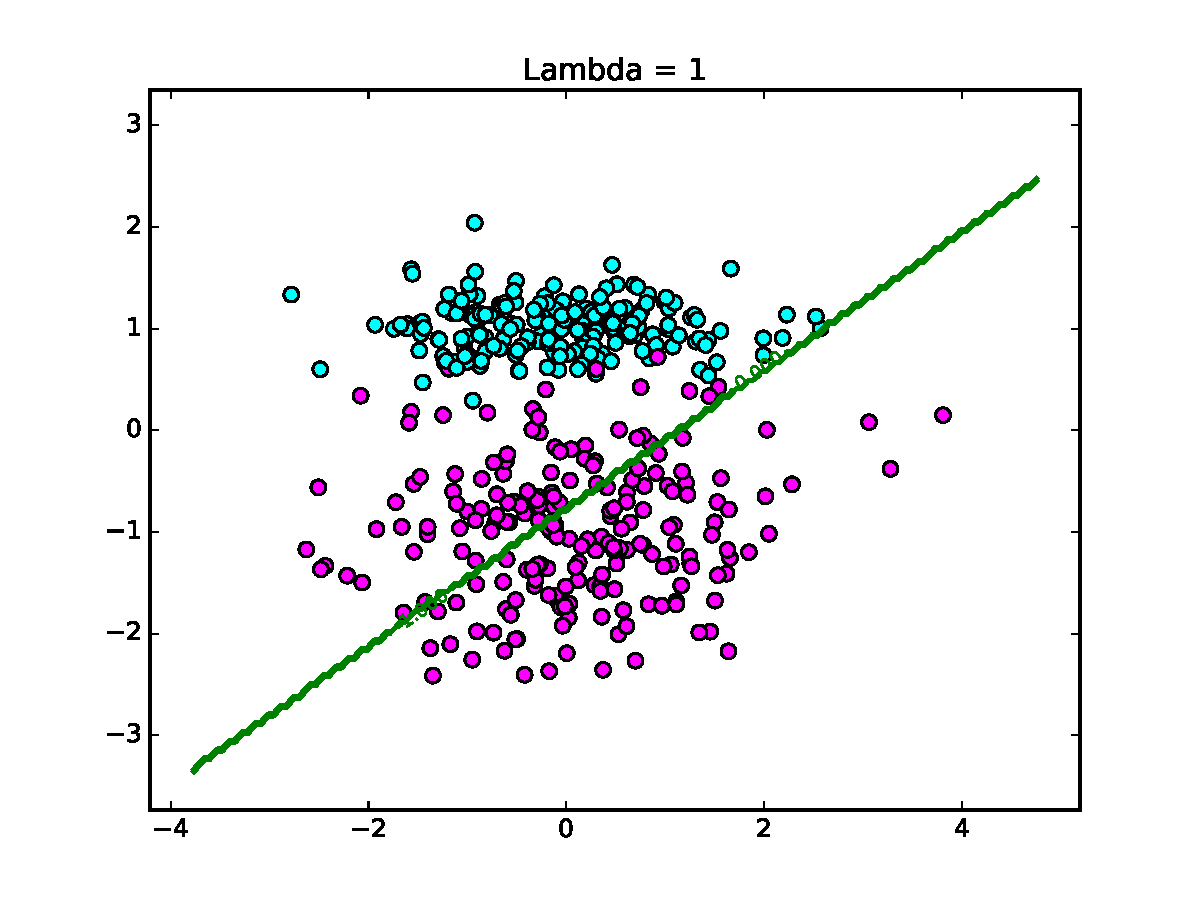
\includegraphics[width=\textwidth]{hw2_3-2_1.pdf}
		\caption{$\lambda = 1$}
	\end{subfigure}
	\caption{(a): Margin sizes with respect to regularization strengths $\lambda$. (b, c, d): Decision boundaries for the training set in artificial dataset 3, with varying regularization strengths.}
\end{figure}

\subsection{Kernelized Soft-SVM for Nonlinear Features} To begin generalizing the Soft-SVM to the case of nonlinear features, we can begin by considering the kernelized version of Soft-SVM, as follows:
$$\min_w \frac{\lambda}{2} \|w\|^2 +  \sum_n [1-y_n(w^T\phi(x_n))]_+ \Rightarrow \max_a \frac{\lambda}{2}\|w\|^2 + \sum_n \left[ 1- \sum_m a_m y_ny_m K(x_n,x_m) \right]_+$$
where the right-hand side is the dual form of the kernelized Soft-SVM with the kernel $K$ explicitly shown, and we have substituted the primal solution $w = \sum_n a_n y_n \phi(x_n)$. By using a modified, corresponding version of the kernelized Pegasos algorithm, we can solve the above maximization problem for the $a$ (Lagrange multiplier) variables and reconstruct the weight vector $w$. More directly, however, we can simply use the kernelized version of the discriminant function as the predictor. That is, for a new point $x$, we can use the fact that:
$$w^T\phi(x) = \sum_n a_n y_n \phi(x_n)^T\phi(x) = \sum_n a_n y_n K(x_n,x)$$
using our output values of $a$ from Pegasos to make the prediction. As we have shown, this formulation is exactly equivalent to the dual C-SVM, so the same sparsity properties apply. Though dependent on the choice of basis function (i.e. kernel), it is expected that the kernelized Soft-SVM will yield relatively sparse solutions in terms of $a$, since the nonzero weights are only placed on support vectors.

\begin{wrapfigure}{L}{0.3\textwidth}
	\centering
	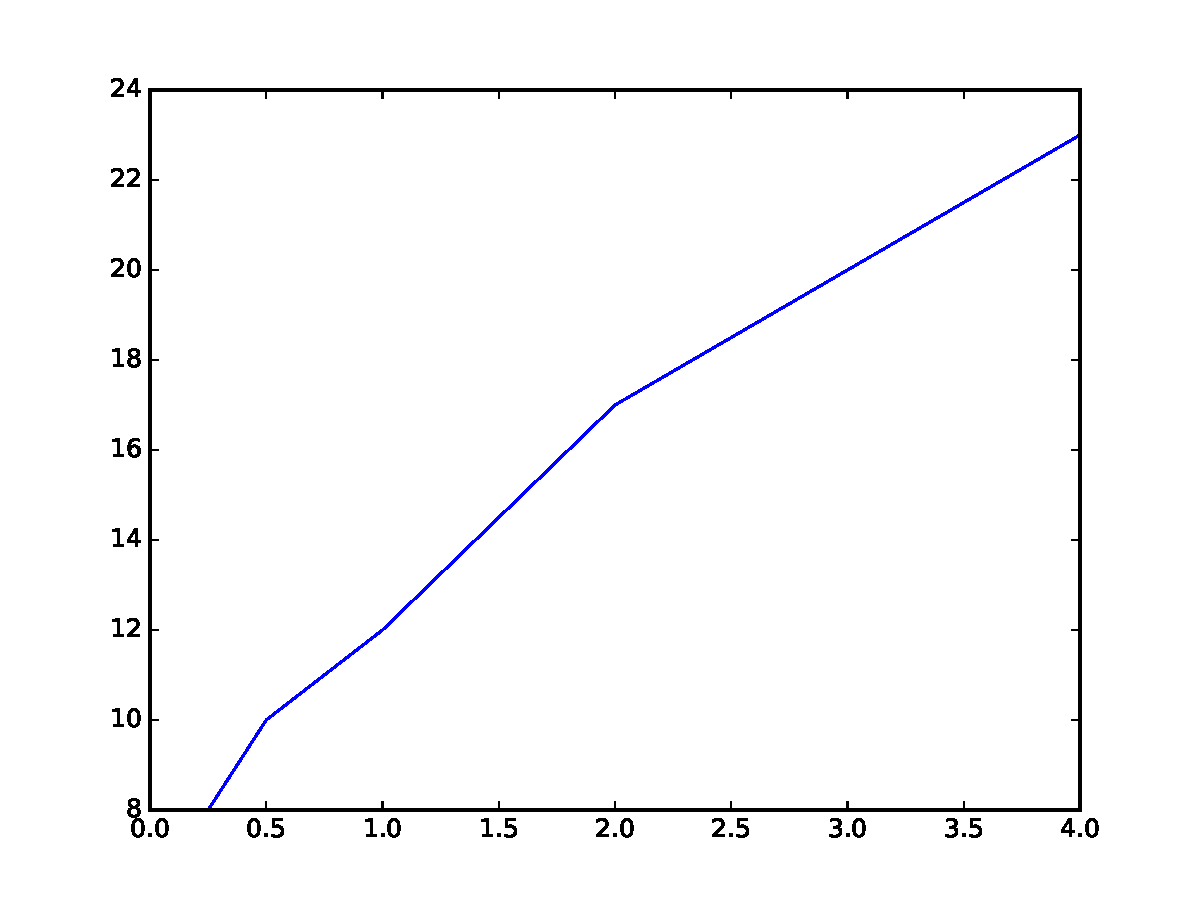
\includegraphics[width=0.23\textwidth]{hw2_3-4_sv.pdf}
	\caption{Number of support vectors as $\gamma$ varies on Soft-SVM.}
\end{wrapfigure}

\subsection{Hyperparameter Dependence of Kernelized Soft-SVM} To demonstrate this behavior, we again return to Gaussian radial basis functions (RBFs) by employing a Gaussian kernel in the kernelized Soft-SVM. We focus on the dependence of the sparsity and decision boundary properties on the choice of kernel, i.e. varying the bandwidth values of the Gaussian kernel, so we fix $\lambda = 0.02$ for all experiments, and instead let $\gamma$ vary from $2^2$ to $2^{-2}$.

As shown in {\bf Figure 8}, the number of support vectors increases monotonically with the kernel bandwidth $\gamma$. This is to be expected, as $\gamma \propto 1/\sigma^2$ for the Gaussian kernel, so as $\gamma$ increases, $\sigma^2$ decreases, and each point $x_n$ in the dataset has less influence on the prediction. Because each point is less influential, we require more points in order to make an effective prediction, which yields the increase in the number of support vectors utilized by the classifier in considering the decision boundary.\\

\section{Handwritten Digit Recognition with MNIST}

We now compare the classifiers considered in this paper, broadly the logistic regression and SVM models, on a real dataset. In particular, we consider the popular MNIST dataset, which contains $28\times 28$ pixel images of handwritten digits from 0-9. These images are represented as a 784-length vector, with each component specifying the grayscale value of each pixel, ranging from 0 to 255. For all experiments, we use 200 examples (total) from each category (i.e. digit '4' or 'even numbers') for the training set, 150 examples for the validation set, and 150 examples for the test set analogously. Namely, to classify the digits '1' and '7', we use 200 examples of handwritten '1' images and 200 examples of '7' images for the training set, and so forth.

In order to obtain an apples-to-apples comparison, we vary the slack penalty $C$ for the C-SVM and use the corresponding regularization term:
$$\lambda \equiv \frac{1}{nC}$$
for the logistic regression model. We also consider both $L_1$ and $L_2$ regularizers for the logistic regression classifier in our experiments.

\subsection{Linear SVM vs. Logistic Regression} We compared a number of potential binary classification problems based on the MNIST dataset. To encompass visually challenging examples, our experiments considered: '1' vs. '7', '3' vs. '5', '4' vs. '9', and the overall 'even' vs. 'odd' example.

Our results are shown in {\bf Figure 9}, where we see that for all examples, all of the classifiers considered achieve perfect classification accuracy on the training set. On the test set, however, though the classifiers generally achieve very high classification accuracy ($> 90\%$), they vary in their performance across hyperparameter settings and datasets. For example, on the '1' vs. '7' task, all classifiers achieve $\geq 99\%$ accuracy on good hyperparameter settings. However, on the '3' vs. '5' task, the linear SVM barely achieves $90\%$ accuracy across all hyperparameter settings, with the logistic regression classifier performing uniformly better on accuracy. However, on tasks such as '4' vs. '9' and 'even' vs. 'odd', the SVM performed better than either logistic regression classifier (especially with $L_1$ regularization) on a number of $C$ settings. In fact, the linear SVM uniformly dominates the $L_2$-regularized logistic regression classifier on the 'even' vs. 'odd' task.

Interestingly, normalizing the images to lie within $[-1,1]$ via a simply linear normalization:
$$\tilde{p}_i = \frac{2\cdot p_i}{255} - 1$$
yields very different results, as demonstrated in {\bf Figure 10}. To start, the classifiers do not necessarily achieve perfect classification accuracy across all parameter settings. It is notable that the $L_2$ logistic classifier and linear SVM dominate the $L_1$ logistic classifier on training performance, but the $L_2$ logistic classifier is approximately dominated by the $L_1$ and SVM classifiers on the test set. Moreover, there is strong dependence on the slack penalty $C$; as expected, lower values of $C$ place less emphasis on the classification accuracy of the training set, and therefore result in lower accuracy particularly for the $L_1$ classifier. However, the generalization provided by a lower $C$ value yields better performance on the test set for the $L_2$-regularized and SVM classifiers, but interestingly not for the $L_1$-regularized classifier.

To understand situations in which the classifiers perform poorly, we examine examples that all of the classifiers failed to classify correctly. {\bf Figure 11} shows one such example from each task. It is interesting to note that there are evident features of each incorrectly classified example that are present in the correctly classified example of the other class. for example, for the '1' vs. '7' task, the incorrectly classified '1' image has a tilted stem, which is reminiscent of the stem of the '7' image below. Thus, it appears that the classifiers do perform reasonably, and even when incorrect make predictions based on a features contained in the other class. 

\begin{figure}[t]
	\centering
	\begin{subfigure}[b]{0.23\textwidth}
		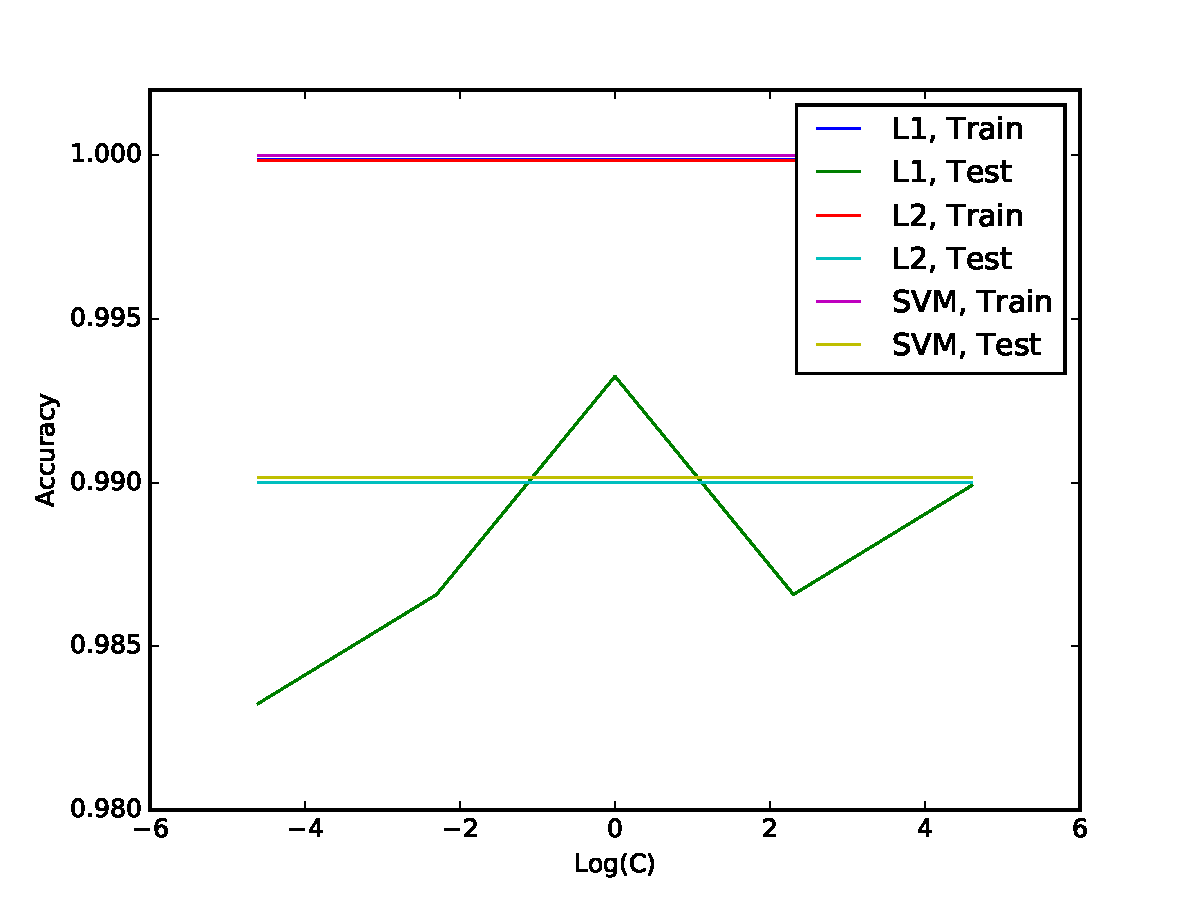
\includegraphics[width=\textwidth]{hw2_4-1_1v7.pdf}
		\caption{'1' vs. '7'}
	\end{subfigure}
	\begin{subfigure}[b]{0.23\textwidth}
		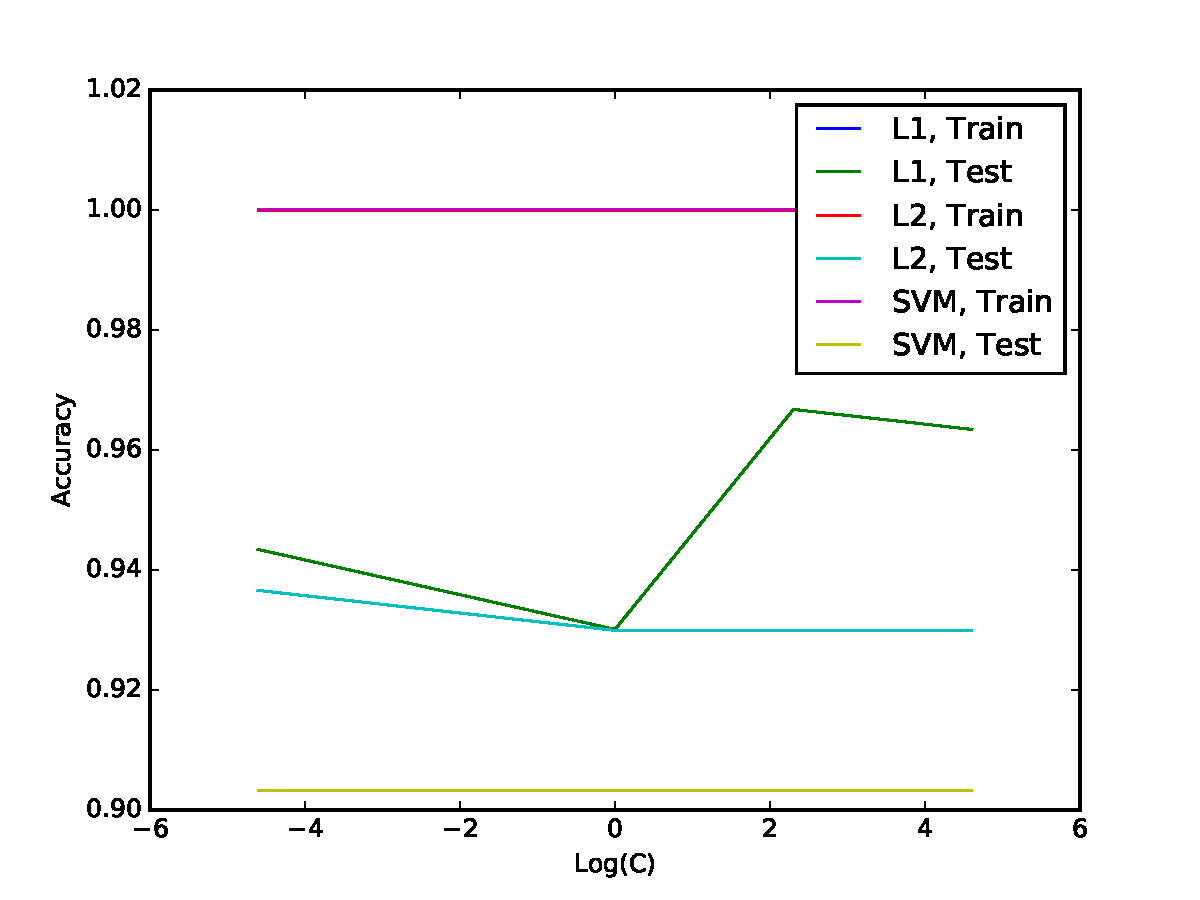
\includegraphics[width=\textwidth]{hw2_4-1_3v5.pdf}
		\caption{'3' vs. '5'}
	\end{subfigure}
	\begin{subfigure}[b]{0.23\textwidth}
		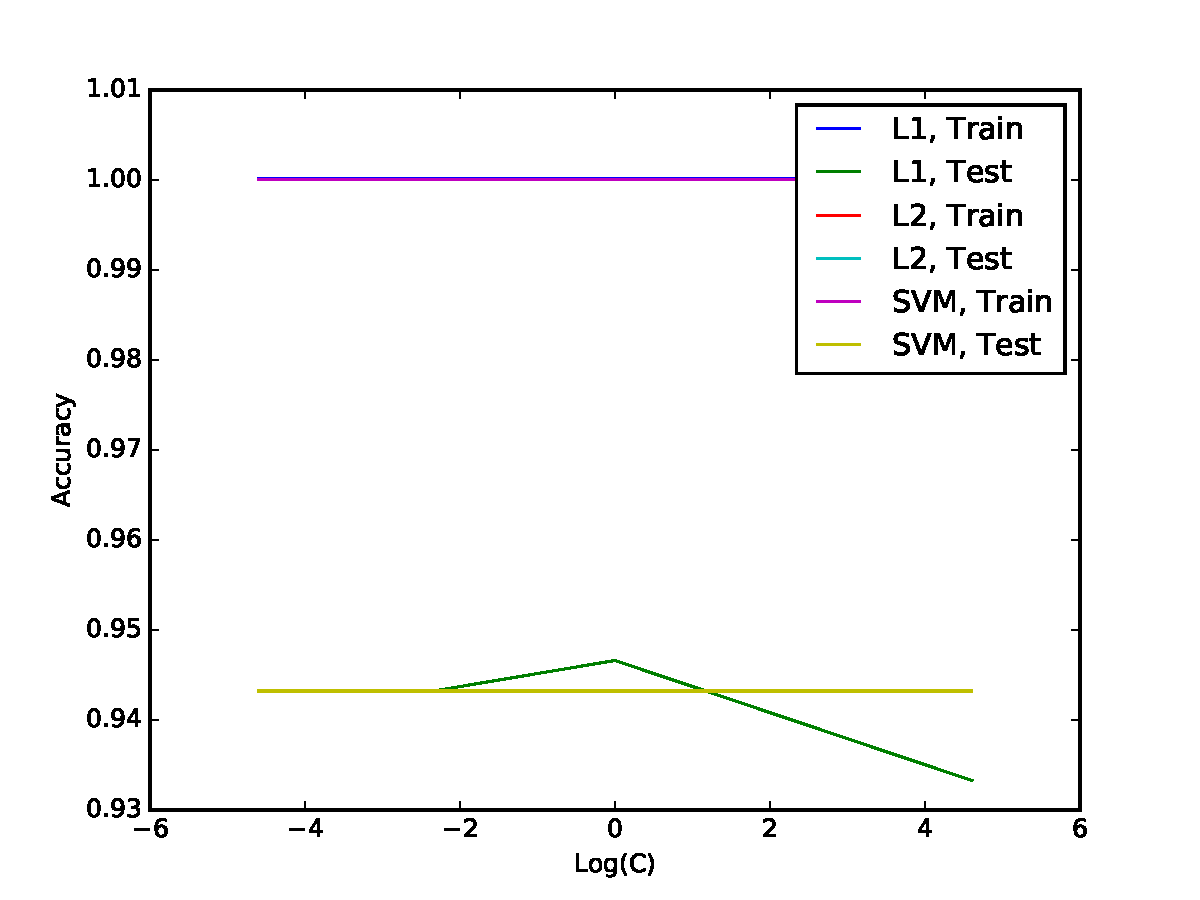
\includegraphics[width=\textwidth]{hw2_4-1_4v9.pdf}
		\caption{'4' vs. '9'}
	\end{subfigure}
	\begin{subfigure}[b]{0.23\textwidth}
		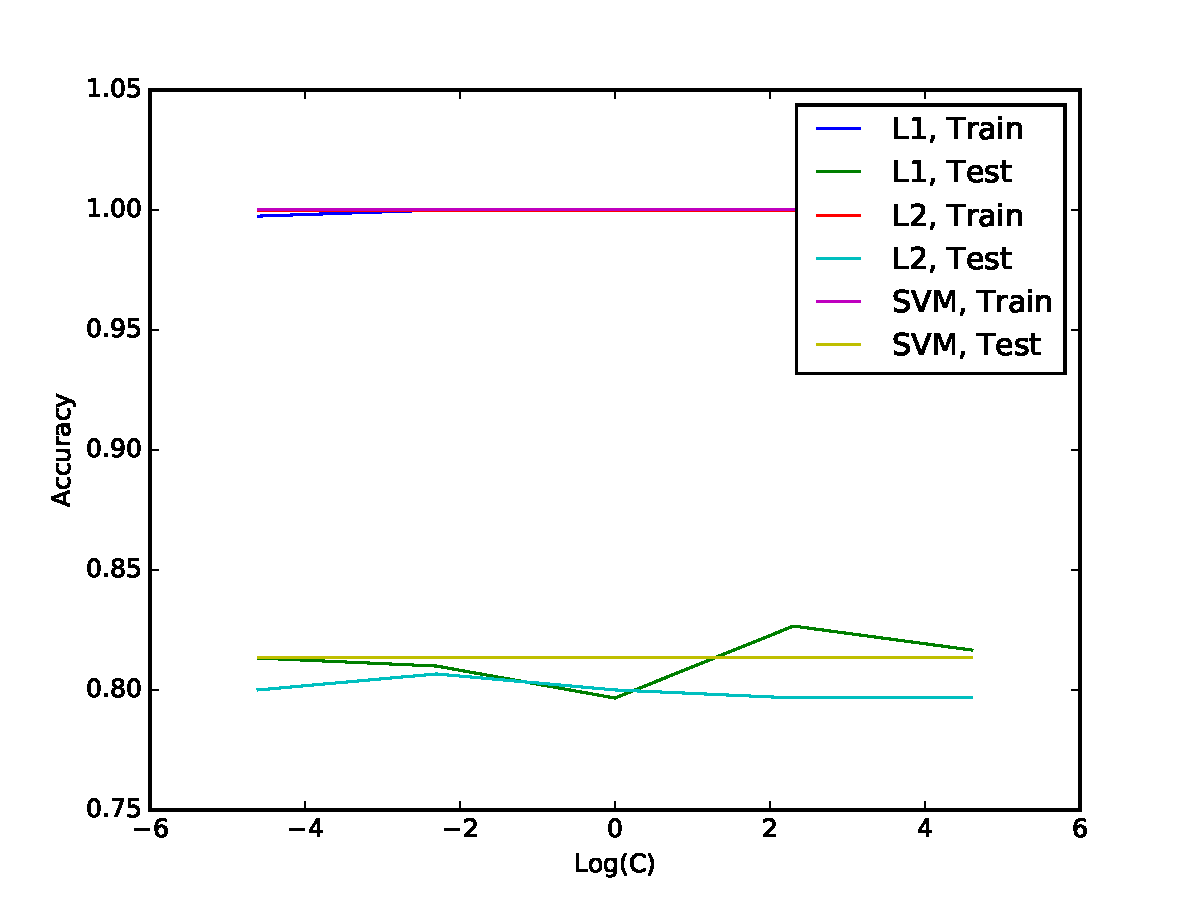
\includegraphics[width=\textwidth]{hw2_4-1_evo.pdf}
		\caption{'Even' vs. 'Odd'}
	\end{subfigure}
	\caption{Classification accuracy on the training and test sets using $L_1$ or $L_2$ logistic regression and linear SVM, for the various binary classification examples given in Section 4.1.}
\end{figure}

\begin{figure}
	\centering
	\begin{subfigure}[b]{0.23\textwidth}
		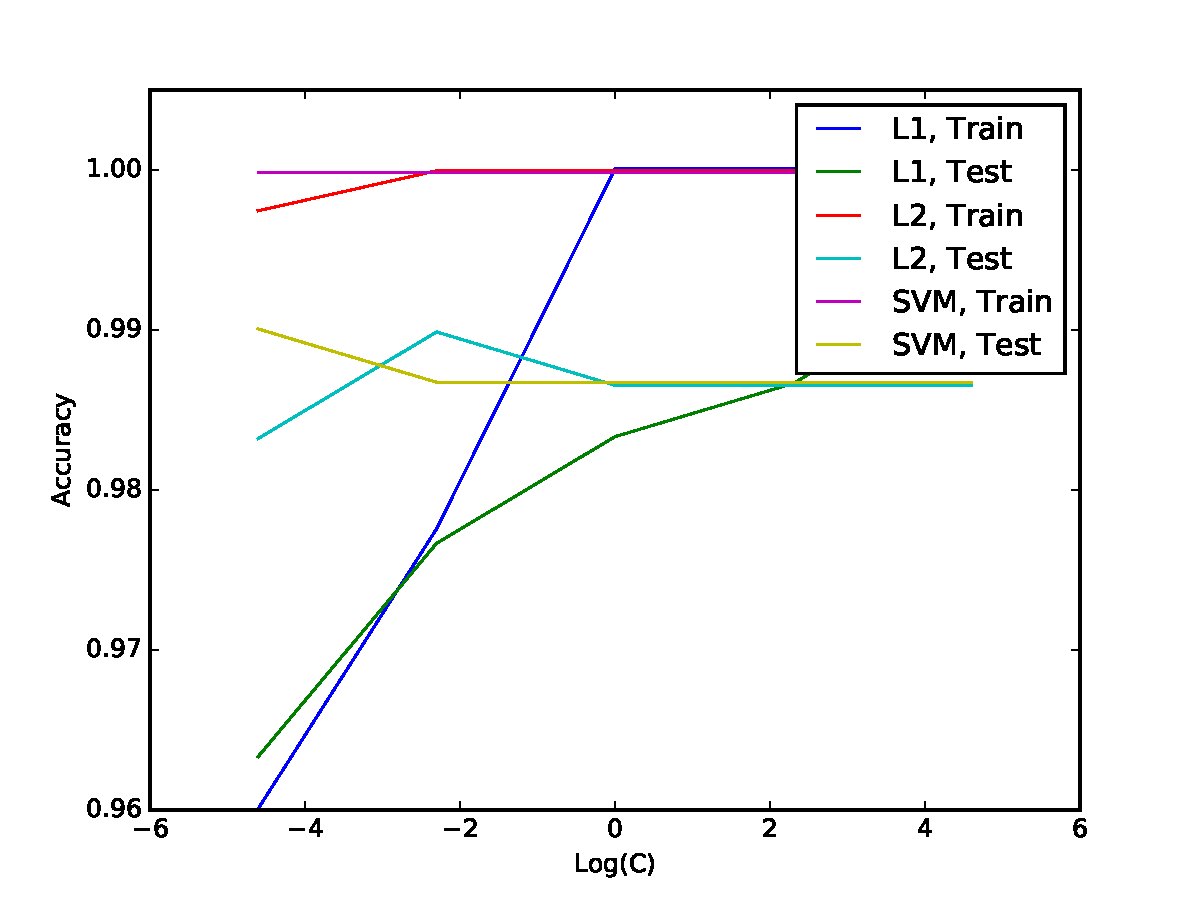
\includegraphics[width=\textwidth]{hw2_4-1_1v7_norm.pdf}
		\caption{'1' vs. '7'}
	\end{subfigure}
	\begin{subfigure}[b]{0.23\textwidth}
		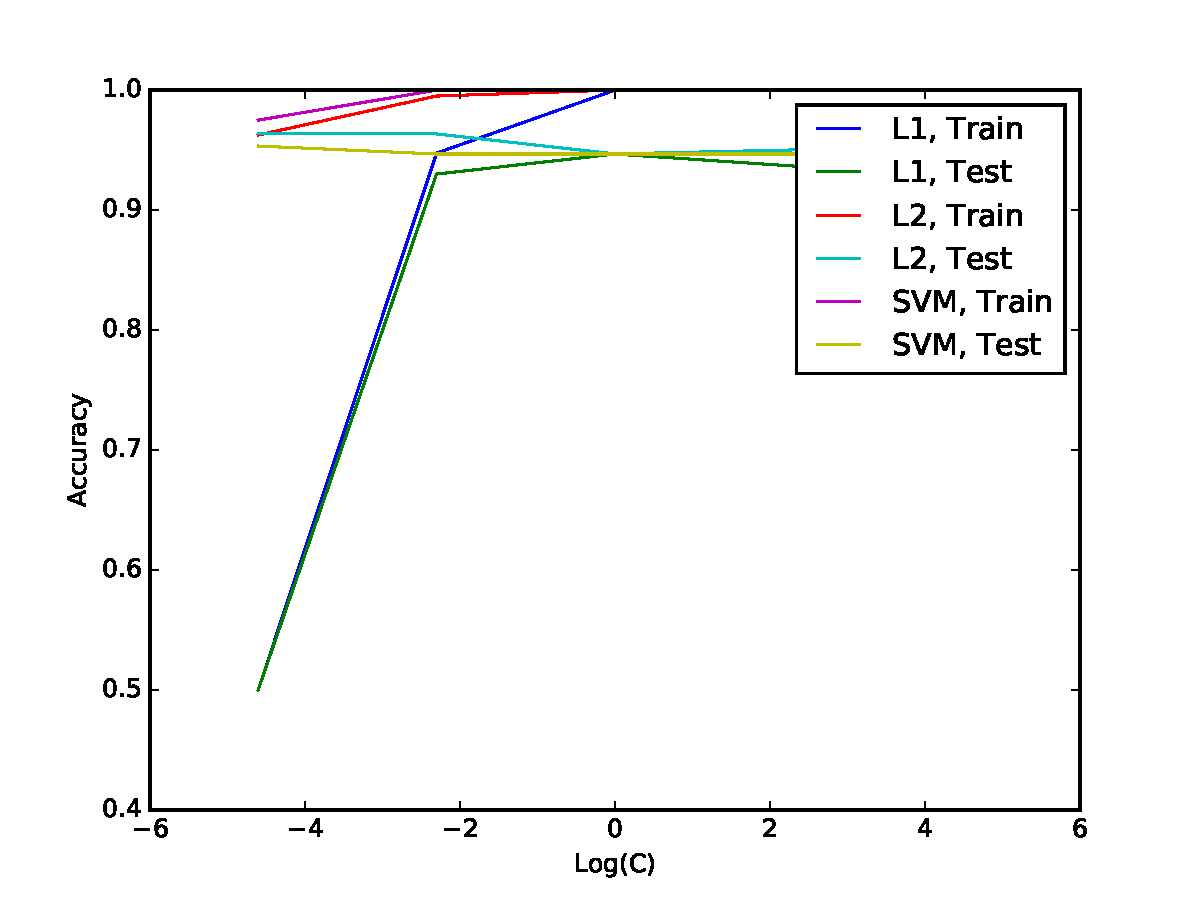
\includegraphics[width=\textwidth]{hw2_4-1_3v5_norm.pdf}
		\caption{'3' vs. '5'}
	\end{subfigure}
	\begin{subfigure}[b]{0.23\textwidth}
		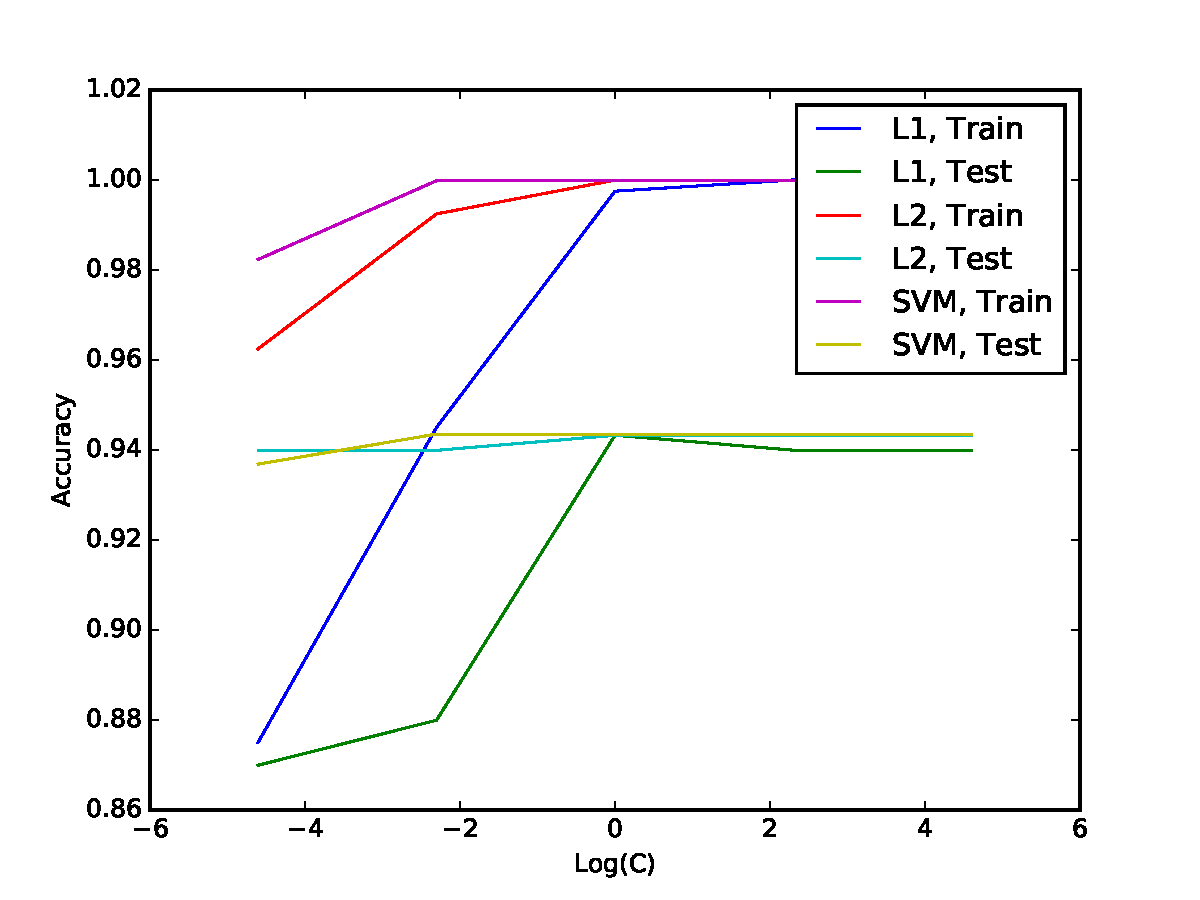
\includegraphics[width=\textwidth]{hw2_4-1_4v9_norm.pdf}
		\caption{'4' vs. '9'}
	\end{subfigure}
	\begin{subfigure}[b]{0.23\textwidth}
		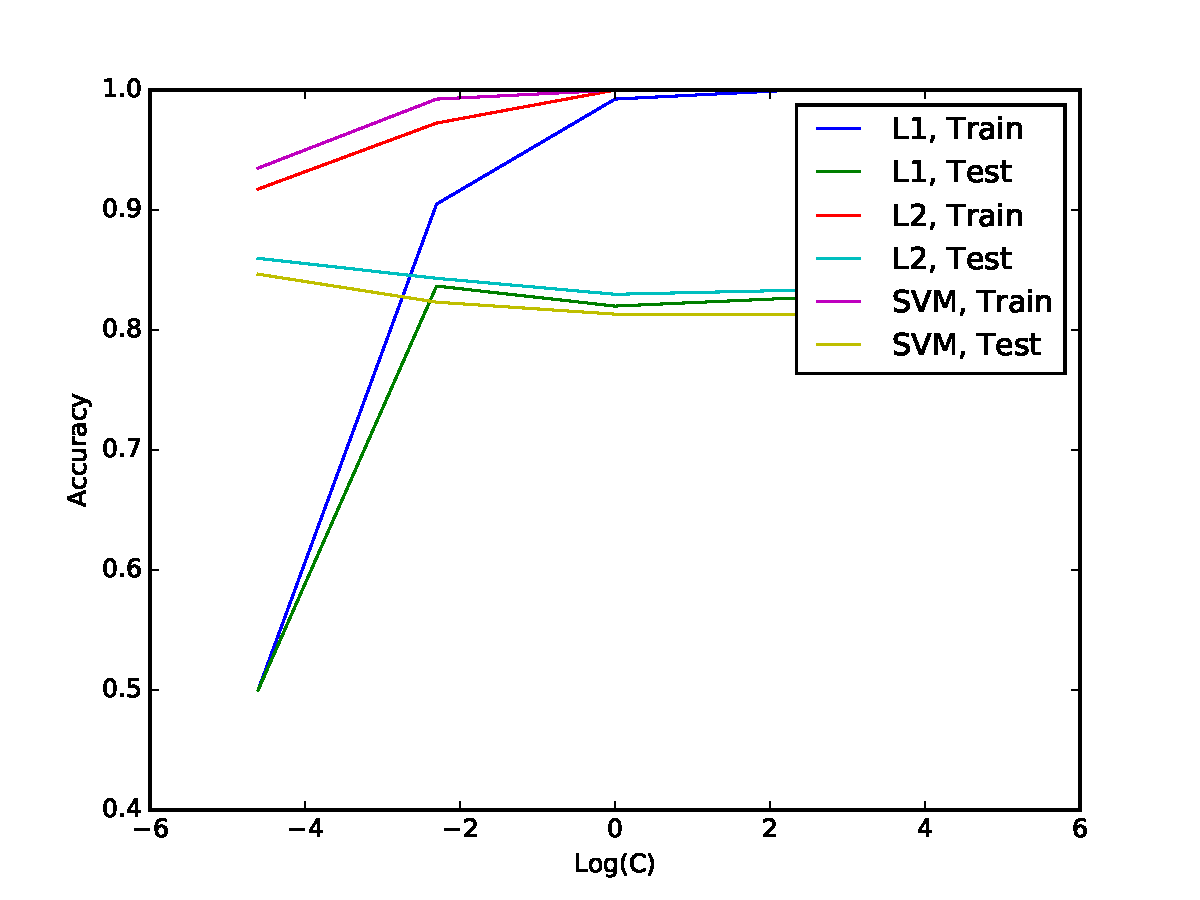
\includegraphics[width=\textwidth]{hw2_4-1_evo_norm.pdf}
		\caption{'Even' vs. 'Odd'}
	\end{subfigure}
	\caption{Classification accuracy with the same setup as in Figure 9, except with normalized images as described in the text.}
\end{figure}

\begin{figure}[b]
	\centering
	\begin{subfigure}[b]{0.25\textwidth}
		\centering
		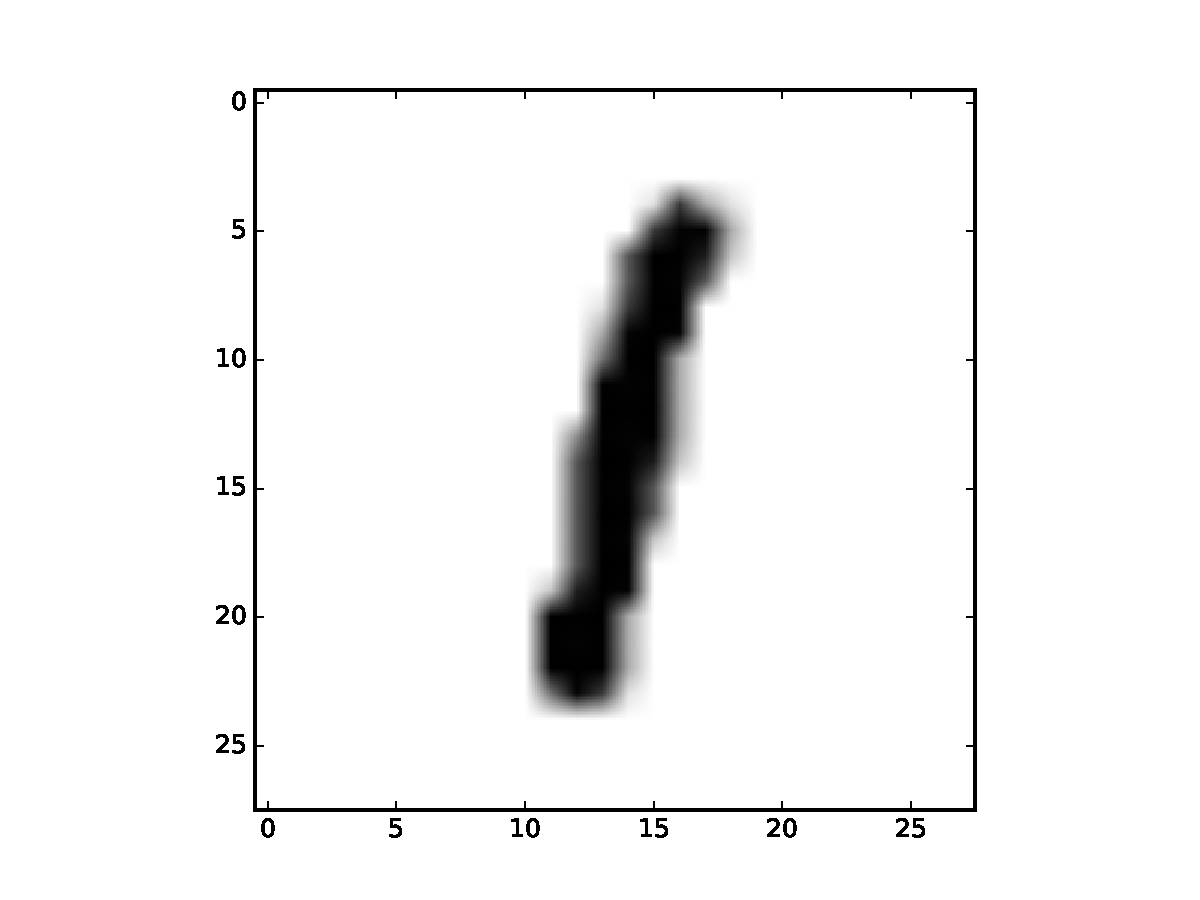
\includegraphics[width=0.6\textwidth]{hw2_4-1_1v7_ex.pdf}
		\caption{'1' Wrong}
	\end{subfigure}
	\begin{subfigure}[b]{0.25\textwidth}
		\centering
		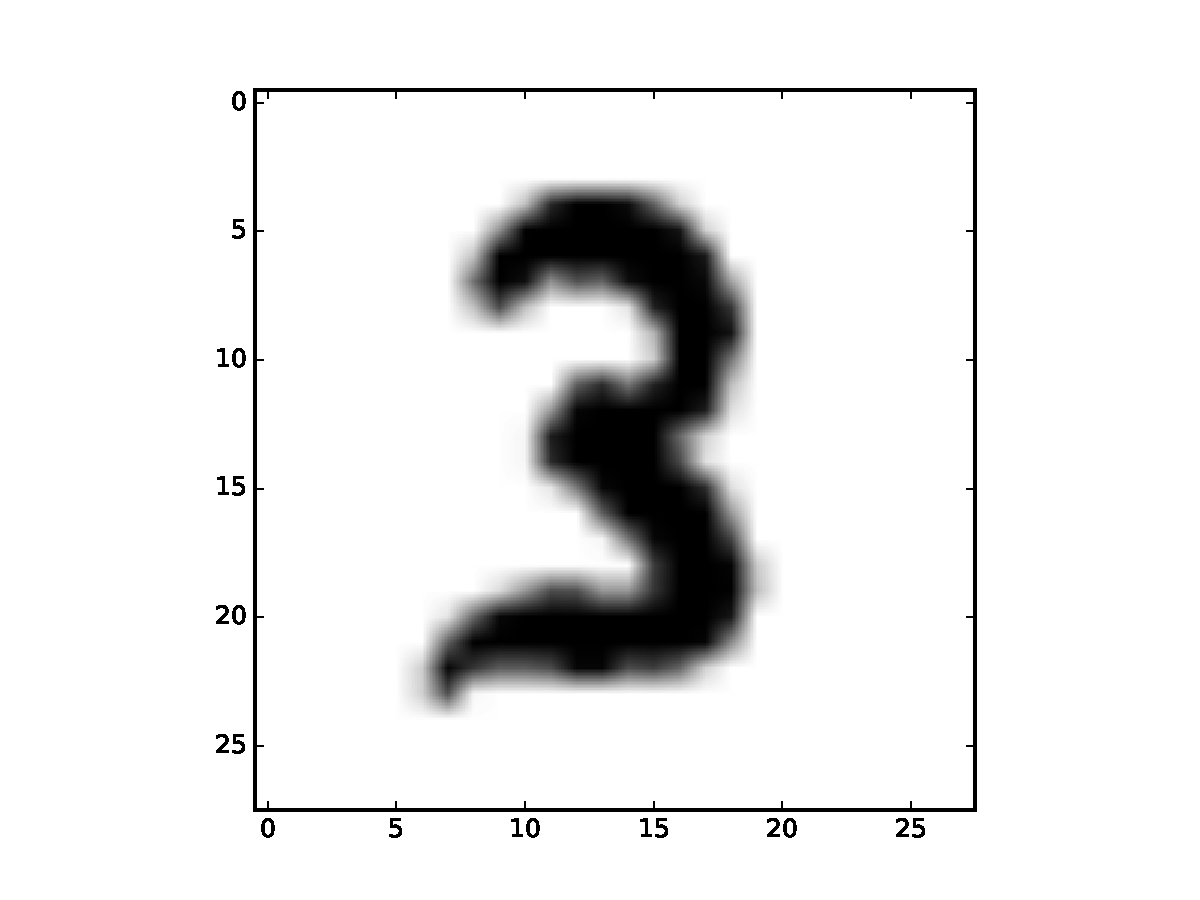
\includegraphics[width=0.6\textwidth]{hw2_4-1_3v5_ex.pdf}
		\caption{'3' Wrong}
	\end{subfigure}
	\begin{subfigure}[b]{0.25\textwidth}
		\centering
		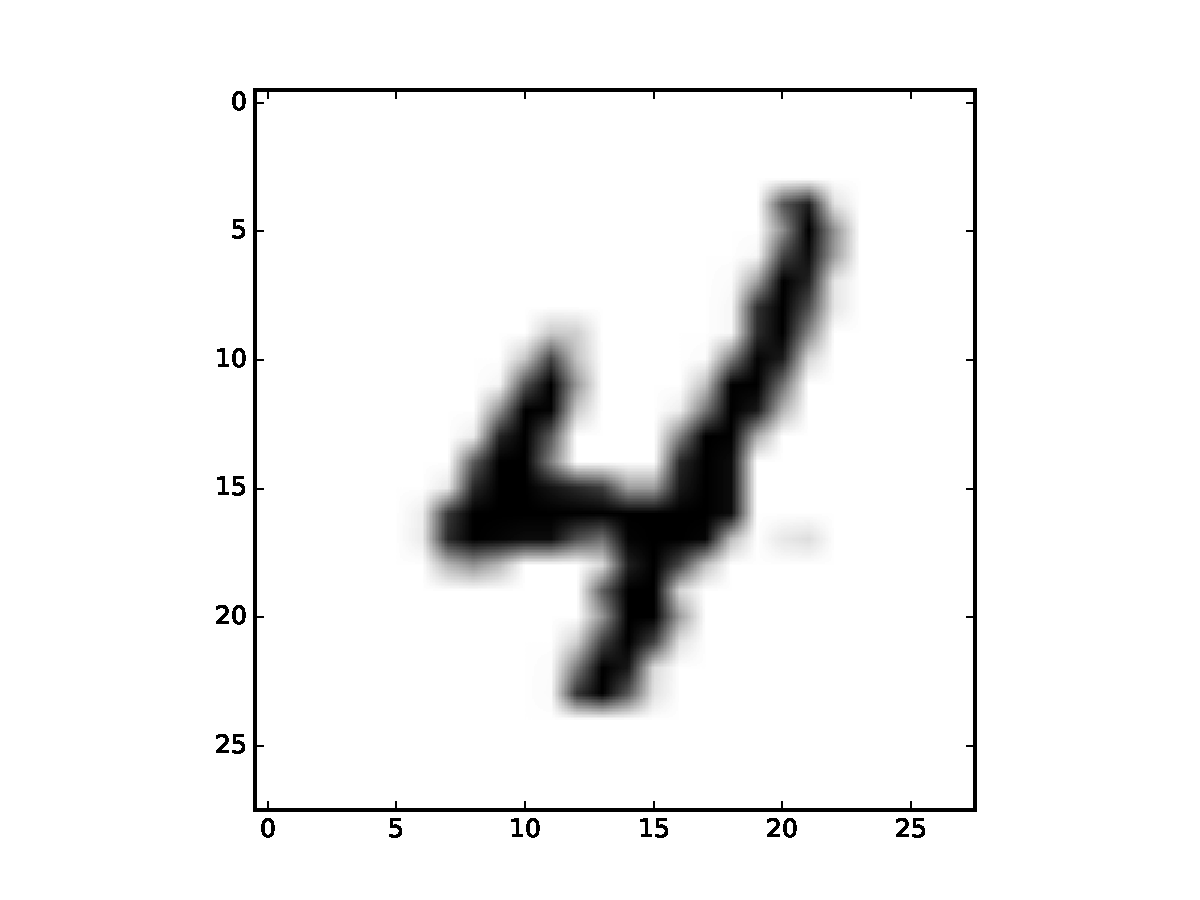
\includegraphics[width=0.6\textwidth]{hw2_4-1_4v9_ex.pdf}
		\caption{'4' Wrong}
	\end{subfigure}
	\begin{subfigure}[b]{0.25\textwidth}
		\centering
		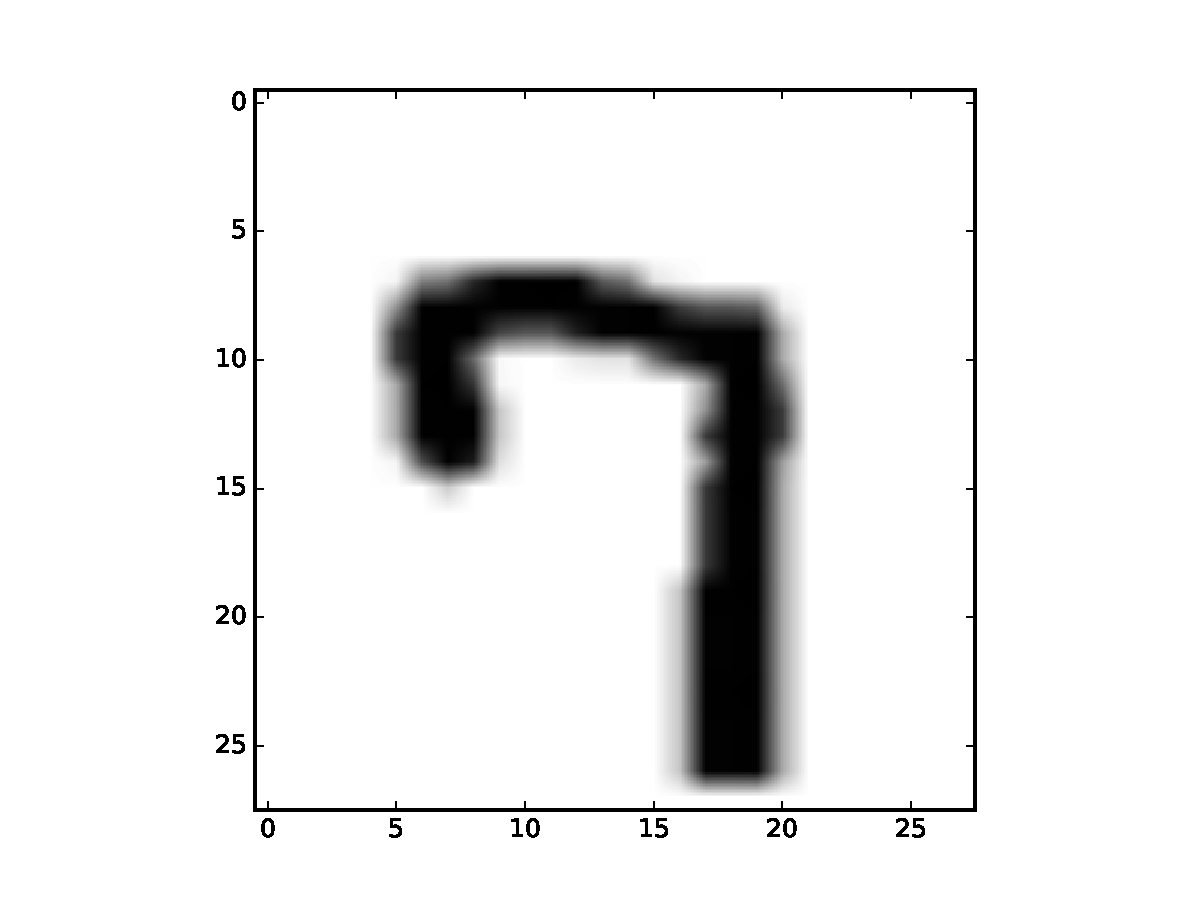
\includegraphics[width=0.6\textwidth]{hw2_4-1_1v7_ex2.pdf}
		\caption{'7' Correct}
	\end{subfigure}
	\begin{subfigure}[b]{0.25\textwidth}
		\centering
		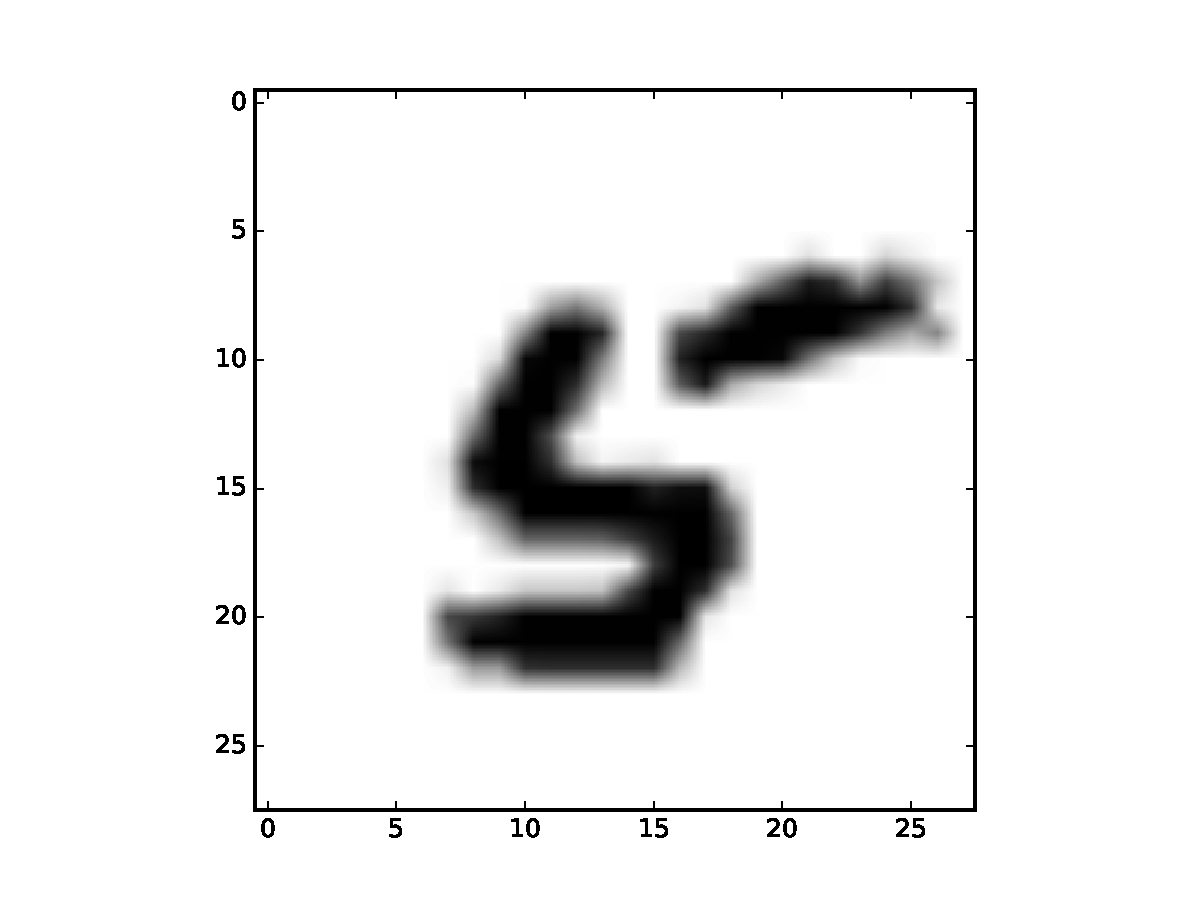
\includegraphics[width=0.6\textwidth]{hw2_4-1_3v5_ex5.pdf}
		\caption{'5' Correct}
	\end{subfigure}
	\begin{subfigure}[b]{0.25\textwidth}
		\centering
		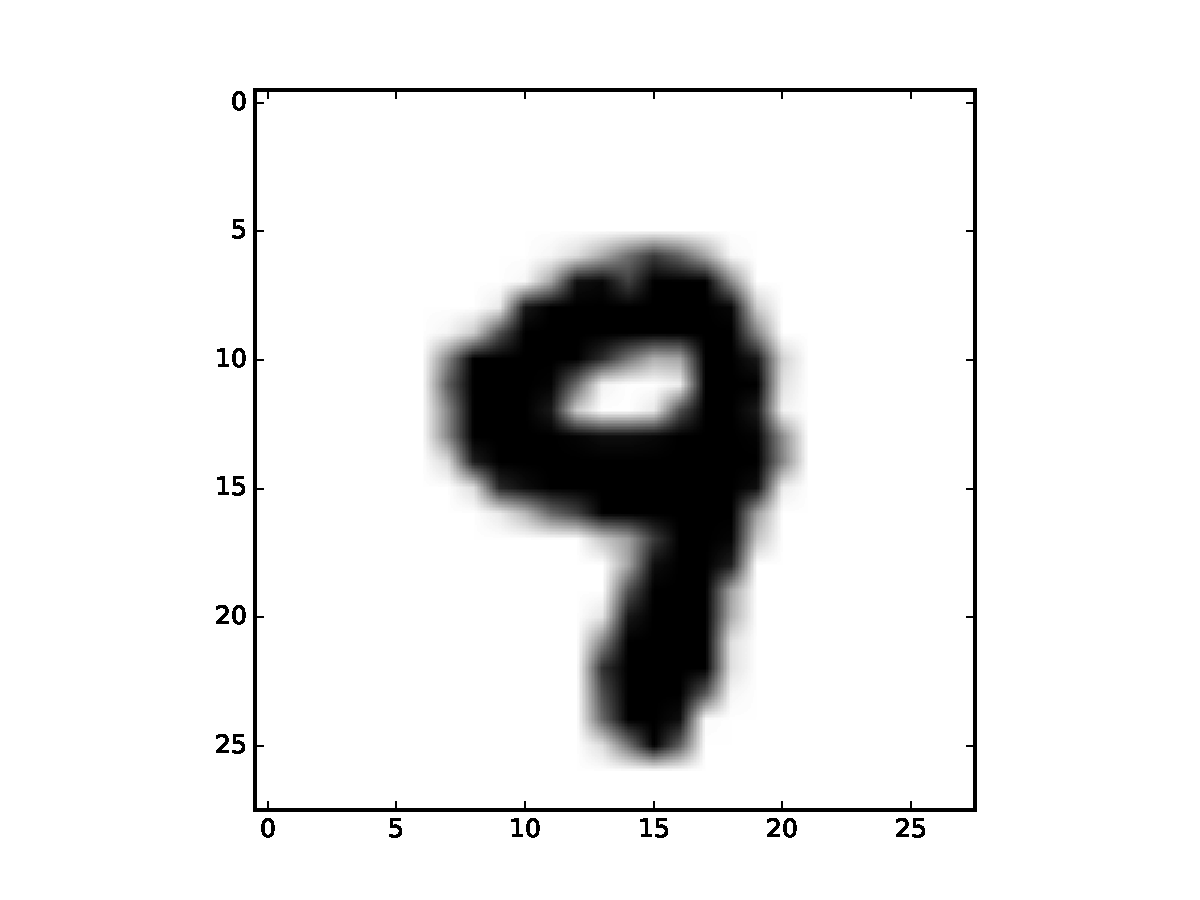
\includegraphics[width=0.6\textwidth]{hw2_4-1_4v9_ex2.pdf}
		\caption{'9' Correct}
	\end{subfigure}
	\caption{Incorrectly classified image for each task by all 3 classifiers, with a correctly classified image of the other class underneath.}
\end{figure}

\subsection{Comparisons with Gaussian RBF Kernel} We further explore the use of nonlinear kernels for the digit classification tasks using the Gaussian RBF kernel. We vary both $C$, the slack penalty, and $\gamma$, the kernel bandwidth; we then train the classifiers on the training set with fixed hyperparameters, and select the hyperparameters that yield the most accurate classifiers on the validation set.

Our results on the validation and test sets are provided in {\bf Figure 12}, where we present the results on the '1' vs. '7' digit task due to space constraints. Interestingly, we find that despite the additional freedom of the $\gamma$ hyperparameter, the Gaussian RBF classifier actually performs worse than the linear classifiers (logistic regression or linear SVM) on both the validation and test sets. Interestingly, this effect is completely nullified (or even reversed) when the images are first normalized, leading all classifiers to achieve near-perfect performance on both the test and validation sets, and the Gaussian RBF classifier to yield marginally better performance on the test set.

\begin{figure}
	\centering
	\begin{subfigure}[b]{0.23\textwidth}
		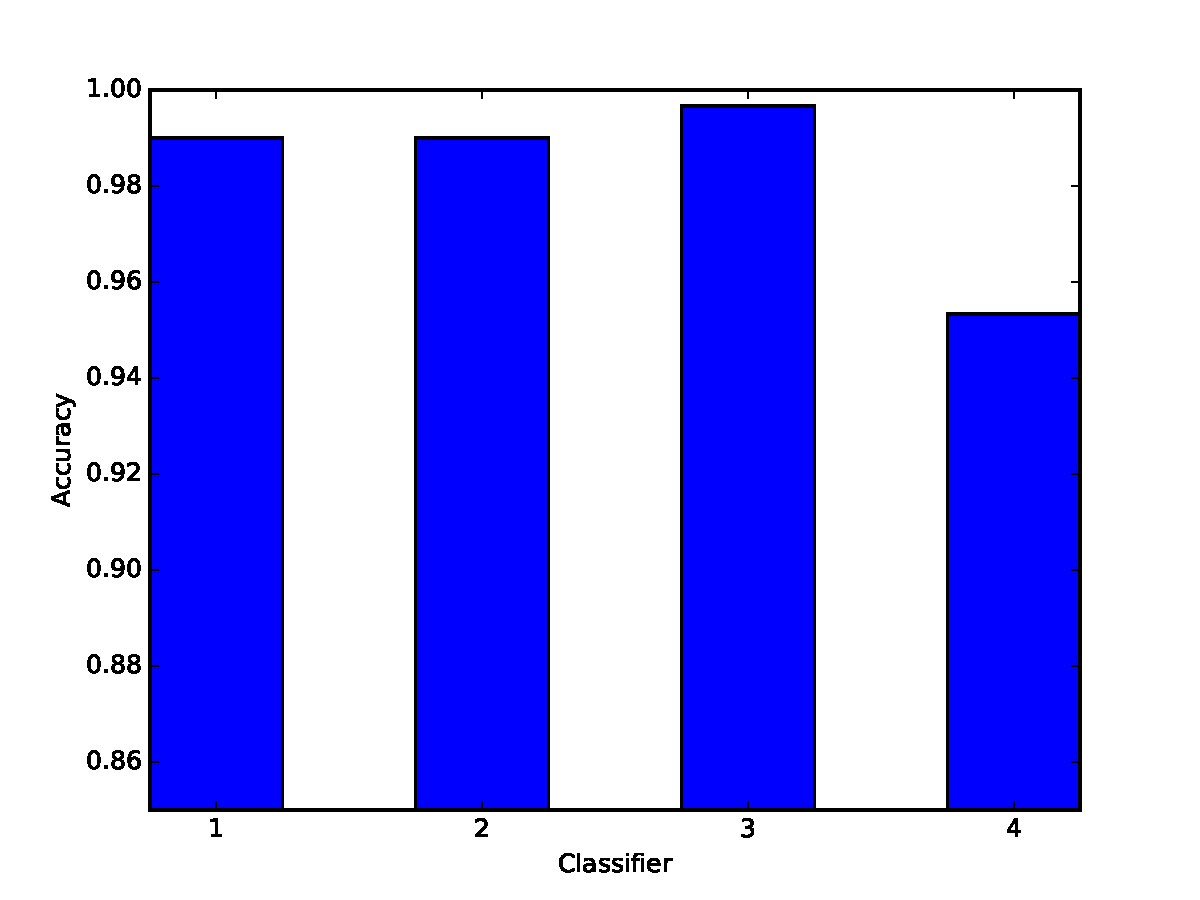
\includegraphics[width=\textwidth]{hw2_4-2_valid.pdf}
		\caption{Validation set}
	\end{subfigure}
	\begin{subfigure}[b]{0.23\textwidth}
		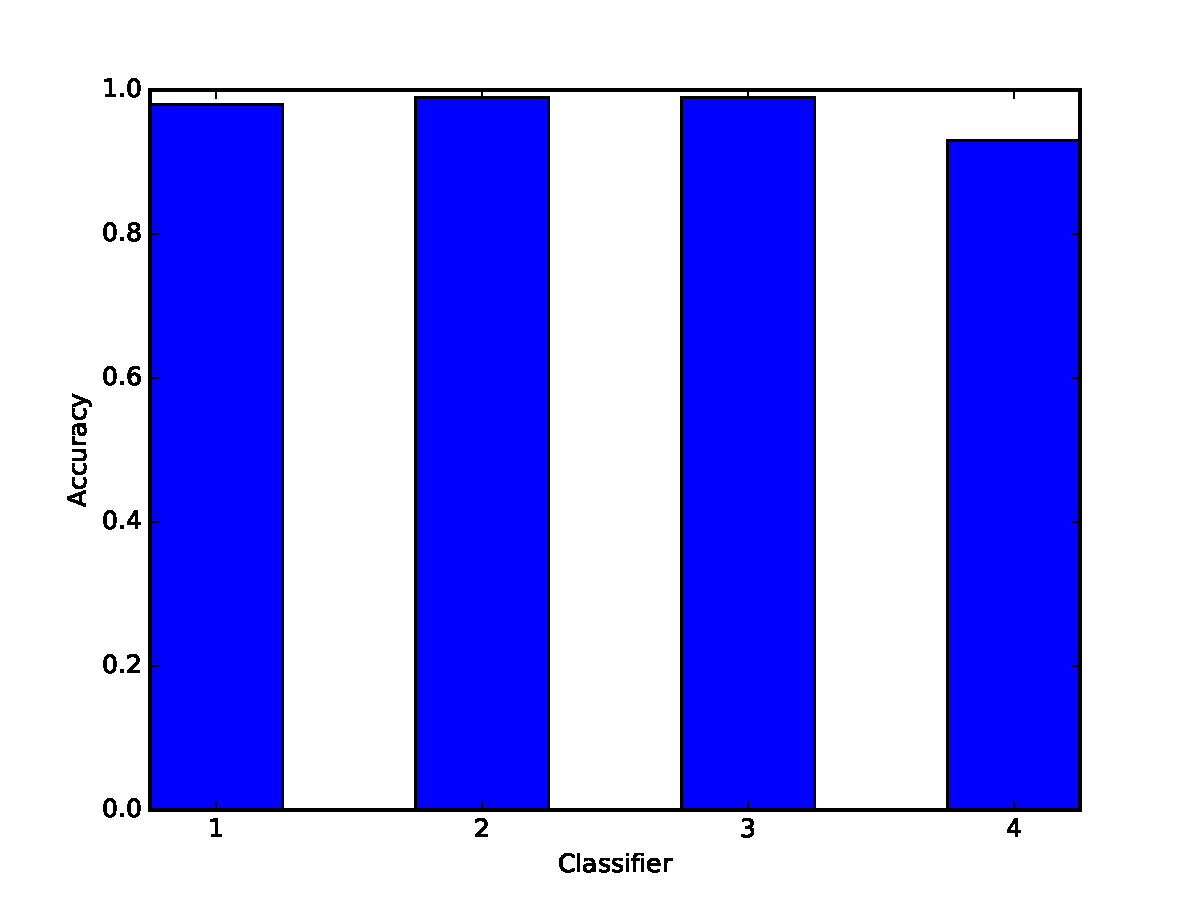
\includegraphics[width=\textwidth]{hw2_4-2_test.pdf}
		\caption{Test set}
	\end{subfigure}
	\begin{subfigure}[b]{0.23\textwidth}
		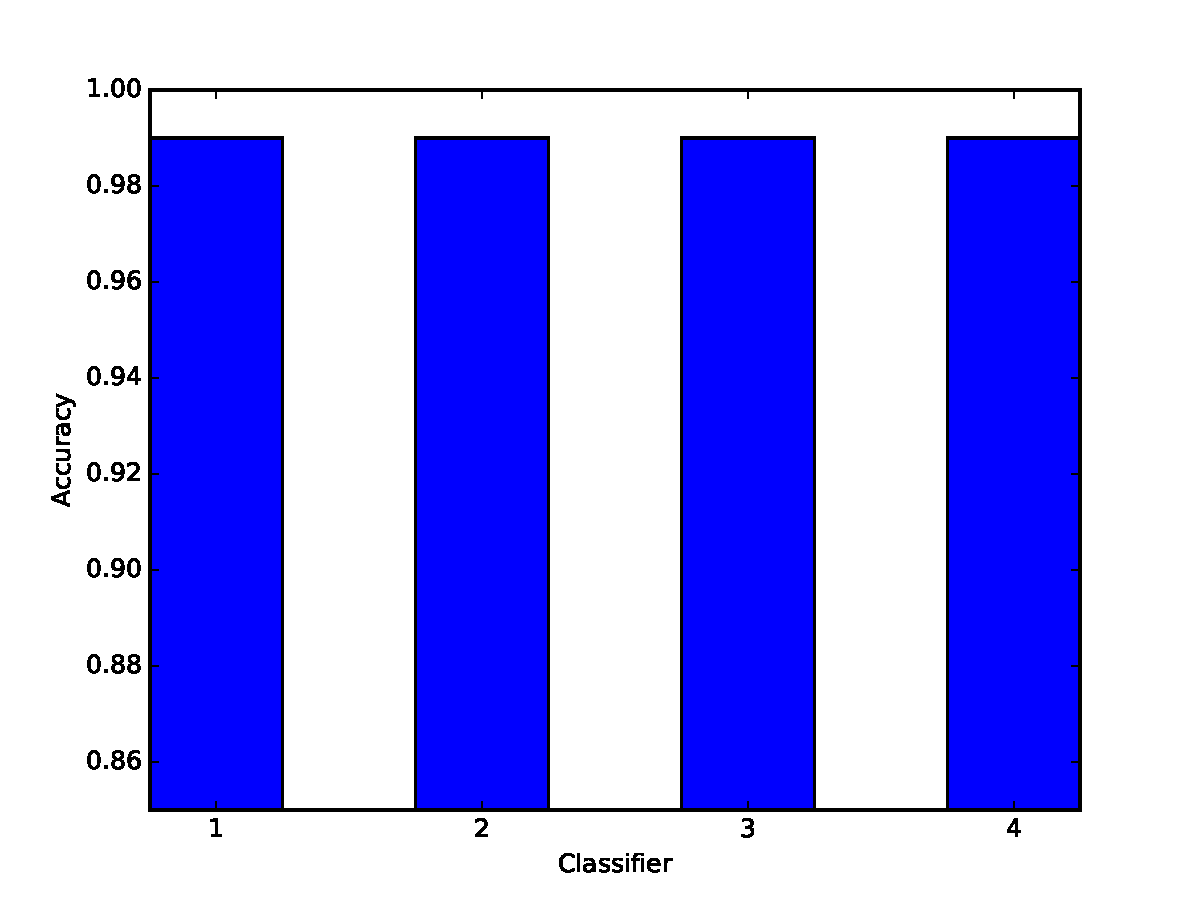
\includegraphics[width=\textwidth]{hw2_4-2_valid_norm.pdf}
		\caption{Valid set (normalized)}
	\end{subfigure}
	\begin{subfigure}[b]{0.23\textwidth}
		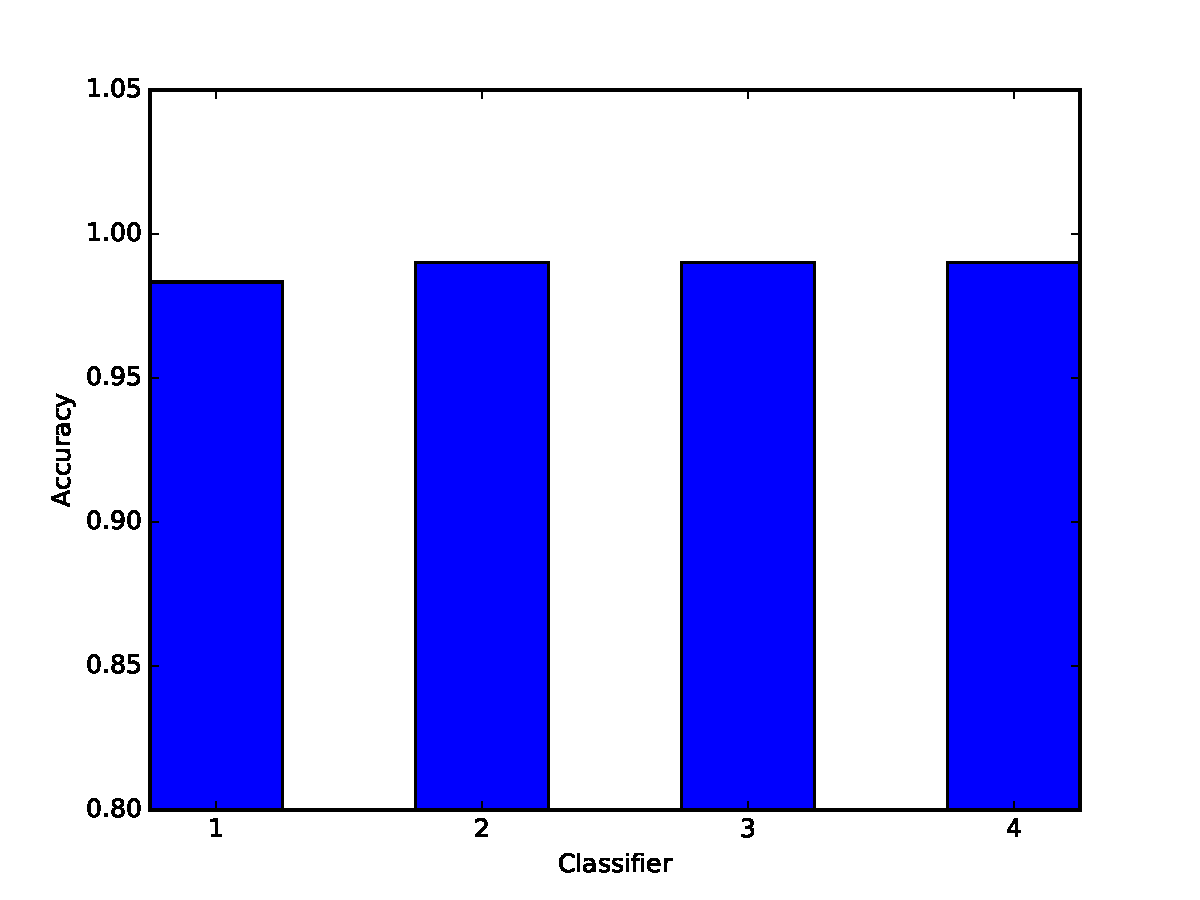
\includegraphics[width=\textwidth]{hw2_4-2_test_norm.pdf}
		\caption{Test set (normalized)}
	\end{subfigure}
	\caption{Results on the test set for classifiers with optimal hyperparameters as evaluated on the validation set: 1 is $L_1$-regularized logistic classifier; 2 is $L_2$-regularized; 3 is the linear SVM; and 4 is the Gaussian RBF kernel SVM.}
\end{figure}

\subsection{Accuracy and Running Times of Pegasos and QP} Finally, we compare the dual C-SVM implementation optimized via the CVX quadratic programming library to the Soft-SVM implementation using Pegasos, in terms of both classification accuracy and running time. We experiment with both linear and Gaussian kernels, and employ the value of the kernel bandwidth $\gamma = 1$ for the Gaussian kernel that was selected on the validation set in the previous experiments.

Our results are illustrated in {\bf Figure 13}, 

\begin{figure}
	\centering
	\begin{subfigure}[b]{0.23\textwidth}
		\includegraphics[width=\textwidth]{hw2_4-3_time.pdf}
		\caption{Running Times}
	\end{subfigure}
	\begin{subfigure}[b]{0.23\textwidth}
		\includegraphics[width=\textwidth]{hw2_4-3_lin.pdf}
		\caption{Linear Kernel Accuracy}
	\end{subfigure}
	\begin{subfigure}[b]{0.23\textwidth}
		\includegraphics[width=\textwidth]{hw2_4-3_gaus.pdf}
		\caption{Gaussian Kernel Accuracy}
	\end{subfigure}
	\caption{(a) Running times for training models via QP or Pegasos. (b) Results on the test set using linear kernels. (c) Results on the test set using Gaussian kernels.}
\end{figure}


\end{document}


